\documentclass[a4paper, 12pt]{article}
\usepackage[utf8]{inputenc}
\usepackage[T1, T2A]{fontenc}
\usepackage[a4paper, top=2cm, bottom=2cm, left=1cm, right=1cm, marginparwidth=1.75cm]{geometry}
\usepackage{graphicx}
\usepackage{amsmath}
\usepackage{amsfonts}
\usepackage{indentfirst}
\usepackage[english, russian]{babel}
\usepackage[section,above,below]{placeins}
\newcommand{\s}[1]{\sigma_{#1}}
\newcommand{\m}[1]{\mu_{#1}}
\newcommand{\E}[2]{e^{#1 #2}}
\newcommand{\sig}[1]{\sqrt{\alpha^2-\kappa_#1^2}}

\begin{document}

\tableofcontents

\newpage

\section{Постановка задачи}
Дана задача для двухслойного волновода (Рис. 1):
$$u=u(x,z): (x,z) \in \mathbb{R}^2 \rightarrow \mathbb{C},$$
\begin{equation} 
    \Delta u + \kappa_i^2 u=0,\ \kappa_i=\omega/c_i,\ i=1,2,
\end{equation}
\begin{equation}
    \mu_1 \frac{\partial u}{\partial z}|_{z=0}=q(x),
\end{equation}
\begin{equation}
    u|_{z=-h_1+\varepsilon}=u|_{z=-h_1-\varepsilon},
\end{equation}
\begin{equation}
    \mu_1 \frac{\partial u}{\partial z}|_{z=-h_1+\varepsilon}=\ \mu_2 \frac{\partial u}{\partial z}|_{z=-h_1-\varepsilon},
\end{equation}
\begin{equation}
    \mu_2 \frac{\partial u}{\partial z}|_{z=-h}=\ 0,\ h=h_1+h_2,
\end{equation}
где $\omega$ -- круговая частота колебаний, $h_i, i=1, 2$ -- толщины слоёв, $c_i, i=1, 2$ -- скорость звука в слоях, $\kappa_i^2=\left(\dfrac{\omega}{c_i} \right)^2, i=1, 2$ -- волновые числа в слоях, $q$ -- нагрузка. Условия типа $ u|_{z=-h_1+\varepsilon}=u|_{z=-h_1-\varepsilon}$ или $ u|_{z=-h_1+0}=u|_{z=-h_1-0}$ означают непрерывность функции $u$ по аргументу $z$ на границе слоёв. В уравнении (2) под $\dfrac{\partial u}{\partial z}$ понимается именно действительная часть этой функции.
\begin{figure}[h!]
\noindent\centering{
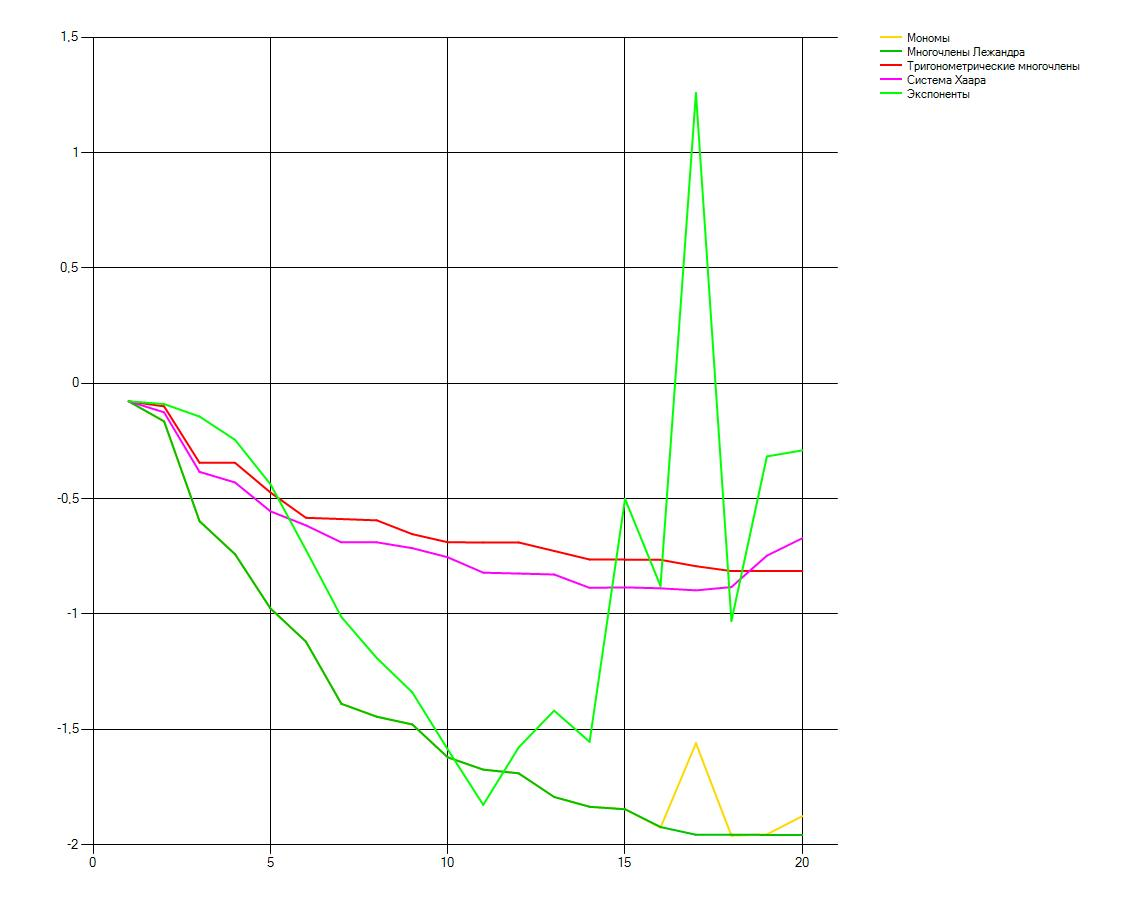
\includegraphics[width=12cm]{1.png}
}
\caption{Геометрия задачи}
\label{figCurves}
\end{figure} 

\section{Полуаналитическое решение}
Сперва построим решения уравнений Гельмгольца. После преобразования Фурье для функции $u(x,z)$ по первому аргументу:

\begin{equation}
    U(\alpha,z)=\int_{-\infty}^{\infty}\ u(x,z) \ e^{i\alpha x} dx,
\end{equation}

получаем обыкновенные дифференциальные уравнения относительно $z$:

$$(-i\alpha)^2 U+U''+\kappa_i^2U=0$$
и граничные условия:

\begin{equation}
   \mu_1 U'|_{z=0}=Q(\alpha), 
\end{equation}

\begin{equation}
    \mu_2  U'|_{z=-h}=\ 0,
\end{equation}

\begin{equation}
    U|_{z=-h_1+\varepsilon}=U|_{z=-h_1-\varepsilon},
\end{equation}

\begin{equation}
    \mu_1  U'|_{z=-h_1+\varepsilon}=\ \mu_2  U'|_{z=-h_1-\varepsilon},
\end{equation}

где $U, Q$ - трансформанты $u, q$ соответственно.

ОДУ $U'' +U (\kappa_i^2-\alpha^2)=0$ имеют общие решения $U=\bar C_1 e^{\sqrt{\kappa_i^2-\alpha^2} z} + \bar C_2 e^{-\sqrt{\kappa_i^2-\alpha^2} z}=C_1 e^{\sqrt{\alpha^2-\kappa_i^2} z} + C_2e^{-\sqrt{\alpha^2-\kappa_i^2}}=U(\alpha,z,\kappa_i,C_1,C_2)$. Объединим решениях двух ОДУ в одно семейство, считая, что для каждой полуплоскости существуют свои пары $C_1,\ C_2$ (то есть имеется матрица $\begin{matrix} C_{11} & C_{12} \\ C_{21} & C_{22} \end{matrix}$), зависящие только от переменной $\alpha$. В таком случае граничные условия (с учётом преобразования Фурье) принимают вид:

    \begin{equation}
    \mu_1 \sqrt{\alpha^2-\kappa_1^2} (C_{11}-C_{12})=Q(\alpha),
    \end{equation}   

    \begin{equation}
    U(\alpha,-h_1+0,\kappa_1,C_{11},C_{12}) = U(\alpha,-h_1-0,\kappa_2,C_{21},C_{22}),
    \end{equation}

    \begin{equation}
    \mu_1 U'(\alpha,-h_1+0,\kappa_1,C_{11},C_{12}) =\mu_2 U'(\alpha,-h_1-0,\kappa_2,C_{21},C_{22}),
    \end{equation}

    \begin{equation}
    \mu_2 \sqrt{\alpha^2-\kappa_2^2} (C_{21} e^{\sqrt{\alpha^2-\kappa_2^2}(-h)}-C_{22}e^{-\sqrt{\alpha^2-\kappa_2^2}(-h)})=0 .
    \end{equation}

Получаем четыре уравнения для четырёх функций $\begin{matrix} C_{11} & C_{12} \\ C_{21} & C_{22} \end{matrix}$; решения функциональной СЛАУ
\begin{multline}
  \begin{pmatrix} 
\m{1}\sig{1} & -\m{1}\sig{1} & 0 & 0 \\
e^{-\sig{1}h_1} & e^{\sig{1}h_1} & -e^{-\sig{2}h_1} & -e^{\sig{2}h_1}\\
\m{1}\sig{1}e^{-\sig{1}h_1} & -\m{1}\sig{1}e^{\sig{1}h_1} & -\m{2}\sig{2}e^{-\sig{2}h_1} & \m{2}\sig{2}e^{\sig{2}h_1}\\
0 & 0 & \m{2}\sig{2}e^{-\sig{2}h} & -\m{2}\sig{2}e^{\sig{2}h}\\
\end{pmatrix}*\\
*\begin{pmatrix} C_{11} \\ C_{12} \\ C_{21} \\ C_{22} \end{pmatrix}=\begin{pmatrix} Q(\alpha) \\ 0 \\ 0 \\ 0 \end{pmatrix}  
\end{multline}
могут быть получены прямым способом; сначала выразим все коэффициенты $C$ относительно $C_{12}$. Из первого уравнения получаем 
$$C_{11}=C_{12}+\frac{Q(\alpha)}{\mu_1 \sqrt{\alpha^2-\kappa_1^2}}.$$
Из второго уравнения:
$$C_{22}=C_{21} e^{2\sqrt{\alpha^2-\kappa_2^2}(-h)}.$$

Если использовать традиционные для такого типа задач обозначения
$$\sigma_i=\sqrt{\alpha^2-\kappa_i^2},\ i=1, 2,$$
и учитывать выражения для $C_{11}$ и $C_{22}$, получаем четыре уравнения (новая форма граничных условий):
\begin{equation}
    C_{11}=C_{12}+\frac{Q(\alpha)}{\m{1} \s{1}},
\end{equation}
\begin{equation}
    C_{22}=C_{21} \E{2\s{2}}{(-h)},
\end{equation}
\begin{equation}
    C_{11} \E{\s{1}}{(-h_1+0)}+ C_{12} \E{-\s{1}}{(-h_1+0)}=C_{21} \E{\s{2}}{(-h_1-0)}+ C_{22} \E{-\s{2}}{(-h_1-0)},
\end{equation}
\begin{equation}
    \m{1}\s{1}\left(C_{11} \E{\s{1}}{(-h_1+0)}- C_{12} \E{-\s{1}}{(-h_1+0)}\right)=\m{2}\s{2}\left(C_{21} \E{\s{2}}{(-h_1-0)}- C_{22} \E{-\s{2}}{(-h_1-0)}\right).
\end{equation}

Применяя результаты первых двух уравнений к третьему, получаем:
$$\left(C_{12}+\frac{Q(\alpha)}{\m{1} \s{1}} \right) \E{\s{1}}{(-h_1+0)}+ C_{12} \E{-\s{1}}{(-h_1+0)}=C_{21} \E{\s{2}}{(-h_1-0)}+ C_{21} \E{2\s{2}}{(-h)} \E{-\s{2}}{(-h_1-0)},$$
откуда $C_{21}$ выражается через $C_{12}$:
\begin{multline}
C_{21}=\frac{C_{12} \left(\E{\s{1}}{(-h_1+0)}+\E{-\s{1}}{(-h_1+0)}\right)+\frac{Q(\alpha)}{\m{1} \s{1}} \E{\s{1}}{(-h_1+0)}}{\E{\s{2}}{(-h_1-0)}+ \E{2\s{2}}{(-h)} \E{-\s{2}}{(-h_1-0)}}= \\
=\frac{2 C_{12} \ch \left(\s{1} (-h_1+0)\right)+\frac{Q(\alpha)}{\m{1} \s{1}} \E{\s{1}}{(-h_1+0)}}{\E{\s{2}}{(-h_1-0)}+ \E{2\s{2}}{(-h)} \E{-\s{2}}{(-h_1-0)}} =\\
=\frac{C_{12}t_1+t_2}{t_3},
\end{multline}
где
$$t_1=2\ch \left(\s{1} (-h_1+0) \right),$$
$$t_2=\frac{Q(\alpha)}{\m{1} \s{1}} \E{\s{1}}{(-h_1+0)},$$
$$t_3=\E{\s{2}}{(-h_1-0)}+ \E{2\s{2}}{(-h)} \E{-\s{2}}{(-h_1-0)} .$$
Запишем четвёртое уравнение, выразив коэффициенты $C_{11}$, $C_{21}$, $C_{22}$ через $C_{12}$:
\begin{multline}
\m{1}\s{1}\left(\left(C_{12}+\frac{Q(\alpha)}{\m{1} \s{1}}\right) \E{\s{1}}{(-h_1+0)}- C_{12} \E{-\s{1}}{(-h_1+0)}\right)= \\
=\m{2}\s{2}\left(\frac{C_{12}t_1+t_2}{t_3} \E{\s{2}}{(-h_1-0)}- \frac{C_{12}t_1+t_2}{t_3}\E{2\s{2}}{(-h)} \E{-\s{2}}{(-h_1-0)} \right),    
\end{multline}
откуда:
\begin{multline}
C_{12} 2 \sh \left(\s{1} (-h_1+0)\right)+ \frac{Q(\alpha)}{\m{1} \s{1}}\E{\s{1}}{(-h_1+0)}=\\
=\frac{\m{2}\s{2}}{\m{1}\s{1}} \left(\frac{C_{12}t_1+t_2}{t_3}\right)\left(\E{\s{2}}{(-h_1-0)}- \E{2\s{2}}{(-h)} \E{-\s{2}}{(-h_1-0)}\right),
\end{multline}
или:
$$C_{12} t_4+t_2=(C_{12} t_1 + t_2)\frac{\m{2}\s{2}}{\m{1}\s{1}} \frac{t_3^-}{t^3},$$
где
$$t_3^-=\E{\s{2}}{(-h_1-0)}- \E{2\s{2}}{(-h)} \E{-\s{2}}{(-h_1-0)},$$
$$t_4=2\sh \left( \s{1} (-h_1+0)\right).$$
Следовательно:
\begin{multline}
    C_{12}=\frac{t_2 \left( \frac{\m{2}\s{2}t_3^-}{\m{1}\s{1}t_3} -1\right)}{t_4-t_1 \frac{\m{2}\s{2}t_3^-}{\m{1}\s{1}t_3}} =\frac{t_2 \left( \m{2}\s{2}t_3^- - \m{1}\s{1}t_3\right)}{t_4 \m{1}\s{1}t_3 - t_1\m{2}\s{2}t_3^-}=\\
    =\frac{\frac{Q(\alpha)}{\m{1} \s{1}} \E{\s{1}}{(-h_1+0)}\left( \m{2}\s{2}t_3^- - \m{1}\s{1}t_3\right)}{2\sh \left( \s{1} (-h_1+0)\right)\m{1}\s{1}t_3 - 2\ch \left( \s{1} (-h_1+0)\right)\m{2}\s{2}t_3^-}=\frac{Q(\alpha)}{\m{1} \s{1}} T,
\end{multline}
где 
$$T=\frac{\E{\s{1}}{(-h_1+0)}\left( \m{2}\s{2}t_3^- - \m{1}\s{1}t_3\right)}{2\sh \left( \s{1} (-h_1+0)\right)\m{1}\s{1}t_3 - 2\ch \left( \s{1} (-h_1+0)\right)\m{2}\s{2}t_3^-}.$$
Тогда для других коэффициентов верно:
$$C_{11}=\frac{Q(\alpha)}{\m{1} \s{1}}(T+1),$$
$$C_{21}=\frac{Q(\alpha)}{\m{1} \s{1}}\frac{(2\ch \left(\s{1}(-h_1+0) \right)T+\E{\s{1}}{(-h_1+0)})}{t_3},$$
$$C_{22}=\frac{Q(\alpha)}{\m{1} \s{1}}\frac{(2\ch \left(\s{1}(-h_1+0) \right)T+\E{\s{1}}{(-h_1+0)})}{t_3}\E{2\s{2}}{(-h)} .$$


Значит,
    \[
U(\alpha,z) =
\begin{cases}
K_1(\alpha,z)Q(\alpha), & \text{если $-h_1\leq z \leq0$;} \\
K_2(\alpha,z)Q(\alpha), & \text{если $-h\leq z \leq-h_1$,}
\end{cases},
\]
где $K_i, i=1, 2$ -- функции Грина:
$$K_1(\alpha,z)=\frac{1}{\m{1}\s{1}}\left((T+1)\E{\s{1}}{z}+T\E{-\s{1}}{z} \right)=\frac{1}{\m{1}\s{1}}T \left(2 \ch (\s{1}z) +\frac{\E{\s{1}}{z}}{T}\right),$$
$$K_2(\alpha,z)=\frac{1}{\m{1} \s{1}}\frac{(2\ch \left(\s{1}(-h_1+0) \right)T+\E{\s{1}}{(-h_1+0)})}{t_3}\left(\E{\s{2}}{z}+ \E{2\s{2}}{(-h)} \E{-\s{2}}{z} \right),$$
запишем также их производные по $z$:
$$K_1'(\alpha,z)=\frac{1}{\m{1}}\left((T+1)\E{\s{1}}{z}-T\E{-\s{1}}{z} \right)=\frac{1}{\m{1}}T \left(2 \sh (\s{1}z) +\frac{\E{\s{1}}{z}}{T}\right),$$
$$K_2'(\alpha,z)=\frac{\s{2}}{\m{1} \s{1}}\frac{(2\ch \left(\s{1}(-h_1+0) \right)T+\E{\s{1}}{(-h_1+0)})}{t_3}\left(\E{\s{2}}{z}- \E{2\s{2}}{(-h)} \E{-\s{2}}{z} \right).$$

\section{Проверка граничных условий}

$$1) \m{1}U'|_{z=0}=\m{1}K_1'(\alpha,z)Q(\alpha)|_{z=0}=\frac{Q(\alpha)}{\s{1}}T \left(2 \sh (\s{1}0) -\frac{-\s{1}\E{\s{1}}{0}}{T}\right)=Q(\alpha),$$

$$2)\m{2}U'|_{z=-h_1-h_2}=\frac{Q(\alpha)}{\m{1} \s{1}}\frac{(2\ch \left(\s{1}(-h_1+0) \right)T+\E{\s{1}}{(-h_1+0)})}{t_3}\left(\E{\s{2}}{(-h)}- \E{2\s{2}}{(-h)} \E{-\s{2}}{(-h)} \right)=0,$$
\begin{multline}
    3)U|_{z=-h_1+0}-U|_{z=-h_1-0}=\frac{Q(\alpha)}{\m{1} \s{1}} ((T+1)\E{\s{1}}{(-h_1+0)}+T\E{-\s{1}}{(-h_1+0)}-\\
    -\frac{(2\ch \left (\s{1}(-h_1+0) \right)T+\E{\s{1}}{(-h_1+0)})}{\E{\s{2}}{(-h_1-0)}+ \E{2\s{2}}{(-h)} \E{-\s{2}}{(-h_1-0)}}(\E{\s{2}}{(-h_1-0)}+ \E{2\s{2}}{(-h)} \E{-\s{2}}{(-h_1-0)}) )=\\
    =\frac{Q(\alpha)}{\m{1} \s{1}} \left(2 \ch (\s{1}(-h_1+0))T +\E{\s{1}}{(-h_1+0)} - 2 \ch (\s{1}(-h_1+0))T-\E{\s{1}}{(-h_1+0)}\right)=0,
\end{multline}

\begin{multline}
    4)\mu_1  U'|_{z=-h_1+0}-\ \mu_2  U'|_{z=-h_1-0}=\frac{Q(\alpha)}{\m{1} \s{1}}*\\
    *( \m{1}\s{1}\left( 2\sh \left(\s{1}(-h_1+0) \right)T+\E{\s{1}}{(-h_1+0)}\right)-\\
    -\m{2}\s{2} \frac{2\ch \left(\s{1}(-h_1+0) \right)T+\E{\s{1}}{(-h_1+0)}}{t_3}\left(\E{\s{2}}{(-h_1-0)}- \E{2\s{2}}{(-h)} \E{-\s{2}}{(-h_1-0)}  \right)))=\\
    =\frac{Q(\alpha)}{\m{1} \s{1}}*\\
    *( T\left(  \m{1}\s{1} 2\sh \left(\s{1}(-h_1+0)\right)-\m{2}\s{2} \frac{2\ch \left(\s{1}(-h_1+0) \right)}{t_3}\left(\E{\s{2}}{(-h_1-0)}- \E{2\s{2}}{(-h)} \E{-\s{2}}{(-h_1-0)}  \right)\right)+\\
    +\m{1}\s{1}\E{\s{1}}{(-h_1+0)}-\m{2}\s{2}\frac{\E{\s{1}}{(-h_1+0)}}{t_3}\left(\E{\s{2}}{(-h_1-0)}- \E{2\s{2}}{(-h)} \E{-\s{2}}{(-h_1-0)}  \right)=\\
    =\frac{Q(\alpha)}{\m{1} \s{1}}*\\
    *\left(T\left( \m{1}\s{1}2\sh (\s{1}(-h_1+0)) -\m{2}\s{2} 2\ch (\s{1}(-h_1+0))\frac{t_3^-}{t_3} \right) +\m{1}\s{1}\E{\s{1}}{(-h_1+0)}-\m{2}\s{2}\E{\s{1}}{(-h_1+0)} \frac{t_3^-}{t_3}\right)=\\
    =\frac{Q(\alpha)}{\m{1} \s{1}}*\\
    *\left(T\frac{\m{1}\s{1}2\sh(\s{1}(-h_1+0))t_3-\m{2}\s{2}2\ch(\s{1}(-h_1+0))t_3^-}{t_3} +  \frac{\m{1}\s{1}\E{\s{1}}{(-h_1+0)}t_3-\m{2}\s{2}\E{\s{1}}{(-h_1+0)}t_3^-}{t_3} \right)=\\
    =\frac{Q(\alpha)\E{\s{1}}{(-h_1+0)}}{\m{1} \s{1}t_3}*\\
    *\left((\m{2}\s{2}t_3^--\m{1}\s{1}t_3)+(\m{1}\s{1}t_3-\m{2}\s{2}t_3^-) \right)=0.
\end{multline}
Следовательно, найденная функция $U(\alpha,z)$ является трансформантой решения исходной задачи.

Поскольку функции $\sqrt{\alpha^2-\kappa_i^2}, i=1, 2$ и $e^z$ непрерывны, $\E{\s{i}}{z}$ непрерывна как сложная функция;
это значит, что $\E{\s{i}}{(-h_1-0)}=\E{\s{i}}{(-h_1+0)}$, поэтому найденные промежуточные функции $t_1, t_2,\dots, T$ могут быть упрощены (отбрасыванием $+0$ и $-0$, раскрытием скобок и учётом чётности и либо нечётности гиперболических функций):
$$t_1=2\ch \left(\s{1} (-h_1) \right)=2\ch \left(\s{1} h_1 \right),$$
$$t_2=\frac{Q(\alpha)}{\m{1} \s{1}} \E{\s{1}}{(-h_1)},$$
$$t_3=\E{\s{2}}{(-h_1)}+ \E{2\s{2}}{(-h)} \E{-\s{2}}{(-h_1)}=\E{\s{2}}{(-h_1)}+ \E{2\s{2}}{(-h)} \E{\s{2}}{(h_1)},$$
$$t_3^-=\E{\s{2}}{(-h_1)}- \E{2\s{2}}{(-h)} \E{-\s{2}}{(-h_1)}=\E{\s{2}}{(-h_1)}- \E{2\s{2}}{(-h)} \E{\s{2}}{(h_1)},$$
$$t_4=2\sh \left( \s{1} (-h_1)\right)=-2\sh \left( \s{1} h_1\right),$$
\begin{multline}
    T=\frac{\E{\s{1}}{(-h_1)}\left( \m{2}\s{2}t_3^- - \m{1}\s{1}t_3\right)}{2\sh \left( \s{1} (-h_1)\right)\m{1}\s{1}t_3 - 2\ch \left( \s{1} (-h_1)\right)\m{2}\s{2}t_3^-}=\\
    =\frac{\E{\s{1}}{(-h_1)}\left( \m{2}\s{2}t_3^- - \m{1}\s{1}t_3\right)}{\E{\s{1}}{(-h_1)}(\m{1}\s{1}t_3-\m{2}\s{2}t_3^-)-\E{\s{1}}{h_1}(\m{1}\s{1}t_3+\m{2}\s{2}t_3^-)}=\\
    =\frac{1}{\frac{\m{1}\s{1}t_3+\m{2}\s{2}t_3^-}{\m{1}\s{1}t_3-\m{2}\s{2}t_3^-} e^{2\s{1}h_1}-1}.
\end{multline}

\section{Упрощение функций Грина}
Зная выражение $T$, где нет гиперболических функций и дробей в числителе и знаменателе, можно существенно упростить функции Грина:
\begin{multline}
    K_1(\alpha,z)=\frac{1}{\m{1}\s{1}}\left((T+1)\E{\s{1}}{z}+T\E{-\s{1}}{z} \right)=\\
    =\frac{1}{\m{1}\s{1}}\frac{-\E{\s{1}}{h_1}\left( \m{2}\s{2}t_3^- + \m{1}\s{1}t_3\right)\E{\s{1}}{z}+\E{-\s{1}}{h_1}\left(\m{2}\s{2}t_3^- - \m{1}\s{1}t_3\right)\E{-\s{1}}{z}}{\E{\s{1}}{(-h_1)}(\m{1}\s{1}t_3-\m{2}\s{2}t_3^-)-\E{\s{1}}{h_1}(\m{1}\s{1}t_3+\m{2}\s{2}t_3^-)}=\\
    =\frac{1}{\m{1}\s{1}}\frac{-\E{-\s{1}}{h_1}(\m{2}\s{2}t_3^--\m{1}\s{1}t_3)\E{-\s{1}}{z}+\E{\s{1}}{h_1}(\m{1}\s{1}t_3+\m{2}\s{2}t_3^-)\E{\s{1}}{z}}
    {\E{-\s{1}}{h_1}(\m{2}\s{2}t_3^--\m{1}\s{1}t_3)+\E{\s{1}}{h_1}(\m{1}\s{1}t_3+\m{2}\s{2}t_3^-)}=\\
    =\frac{1}{\m{1}\s{1}}\frac{(\m{1}\s{1}t_3+\m{2}\s{2}t_3^-)\E{\s{1}}{(z+h_1)}-(\m{2}\s{2}t_3^--\m{1}\s{1}t_3)\E{-\s{1}}{(z+h_1)}}{\E{-\s{1}}{h_1}(\m{2}\s{2}t_3^--\m{1}\s{1}t_3)+\E{\s{1}}{h_1}(\m{1}\s{1}t_3+\m{2}\s{2}t_3^-)}=\\
    =2*\frac{\m{1}\s{1}t_3\ch(\s{1}(z+h_1))+\m{2}\s{2}t_3^-\sh(\s{1}(z+h_1))}{\m{1}\s{1}\Delta},
    \end{multline}
    \begin{multline}
        K_2(\alpha,z)=\frac{1}{\m{1} \s{1}}\frac{2\ch(\s{1}h_1) T+\E{-\s{1}}{h_1}}{t_3}\left(\E{\s{2}}{z}+ \E{2\s{2}}{(-h)} \E{-\s{2}}{z} \right)=\\
        =\frac{1}{\m{1}\s{1}}
        \frac{(\m{2}\s{2}t_3^--\m{1}\s{1}t_3)+e^{-2\s{1}h_1}(\m{2}\s{2}t_3^--\m{1}\s{1}t_3)+e^{-2\s{1}h_1}(\m{1}\s{1}t_3-\m{2}\s{2}t_3^-)-(\m{1}\s{1}t_3+\m{2}\s{2}t_3^-)}
        {\E{\s{1}}{(-h_1)}(\m{1}\s{1}t_3-\m{2}\s{2}t_3^-)-\E{\s{1}}{h_1}(\m{1}\s{1}t_3+\m{2}\s{2}t_3^-)}*\\
        *\left(\E{\s{2}}{z}+ \E{2\s{2}}{(-h)} \E{-\s{2}}{z} \right)=\frac{-2}{\E{\s{1}}{(-h_1)}(\m{1}\s{1}t_3-\m{2}\s{2}t_3^-)-\E{\s{1}}{h_1}(\m{1}\s{1}t_3+\m{2}\s{2}t_3^-)}\left(\E{\s{2}}{z}+ \E{2\s{2}}{(-h)} \E{-\s{2}}{z} \right)=\\
        =\frac{2\left(\E{\s{2}}{z}+ \E{2\s{2}}{(-h)} \E{-\s{2}}{z} \right)}{\Delta}=\frac{2e^{-\s{2}h}(e^{\s{2}(z+h)}+e^{-\s{2}(z+h)})}{\Delta}=\frac{4e^{-\s{2}h}\ch (\s{2}(z+h))}{\Delta},
    \end{multline}
где $\Delta=\E{-\s{1}}{h_1}(\m{2}\s{2}t_3^--\m{1}\s{1}t_3)+\E{\s{1}}{h_1}(\m{1}\s{1}t_3+\m{2}\s{2}t_3^-)$.

А если учесть, что
$$t_3=\E{\s{2}}{(-h_1)}+ \E{2\s{2}}{(-h)} \E{\s{2}}{(h_1)}=e^{-\s{2}h}(e^{\s{2}h}e^{\s{2}(-h_1)}+e^{-\s{2}h}e^{\s{2}h_1})=2e^{-\s{2}h}\ch(\s{2}(h-h_1)),$$
$$t_3^-=2e^{-\s{2}h}\sh(\s{2}(h-h_1)),$$
получим:
$$K_1(\alpha,z)=2*\frac{\m{1}\s{1}\ch(\s{2}(h-h_1))\ch(\s{1}(z+h_1))+\m{2}\s{2}\sh(\s{2}(h-h_1))\sh(\s{1}(z+h_1))}{\mu_1 \sigma_1 \Delta},$$
$$K_2(\alpha,z)=2*\frac{\ch(\s{2}(z+h))}{\Delta},$$
$$\Delta=\E{-\s{1}}{h_1}(\m{2}\s{2}\sh(\s{2}(h-h_1))-\m{1}\s{1}\ch(\s{2}(h-h_1)))+\E{\s{1}}{h_1}(\m{1}\s{1}\ch(\s{2}(h-h_1))+\m{2}\s{2}\sh(\s{2}(h-h_1))) .$$

На самом деле функции Грина можно ещё сократить на двойку, приведя в знаменателе экспоненты к гиперболическим функциям, но пользы в этом нет.

\section{Численная проверка граничных условий}
Теперь проверим решение численно. В качестве нагрузки $q$ возьмём функцию
\[
q(x) = \delta (x_0-x).
\]
Её трансформанта:
\begin{equation}
  Q(\alpha)= e^{i \alpha x_0}.  
\end{equation}

Поскольку трансформанты являются функциями комплексного переменного, а в каждом из четырёх граничных условий устанавливается равенство между двумя функциями комплексного переменного, сравнивать их будем по модулю (чтобы не нагромождать график множеством кривых, которые должны накладываться друг на друга). Параллельно будем проверять условия для образов этих трансформант (найденных численно обратным преобразованием Фурье), которые являются функциями тоже комплексного переменного (сравнение ведётся по действительной части). В следующих примерах зафиксированы параметры: $c_1=1, c_2=2, h_1=h_2=1, \mu_1=1, \mu_2=1.6, \omega=2, x_0=1$.

\begin{figure}[h!]
\noindent\centering{
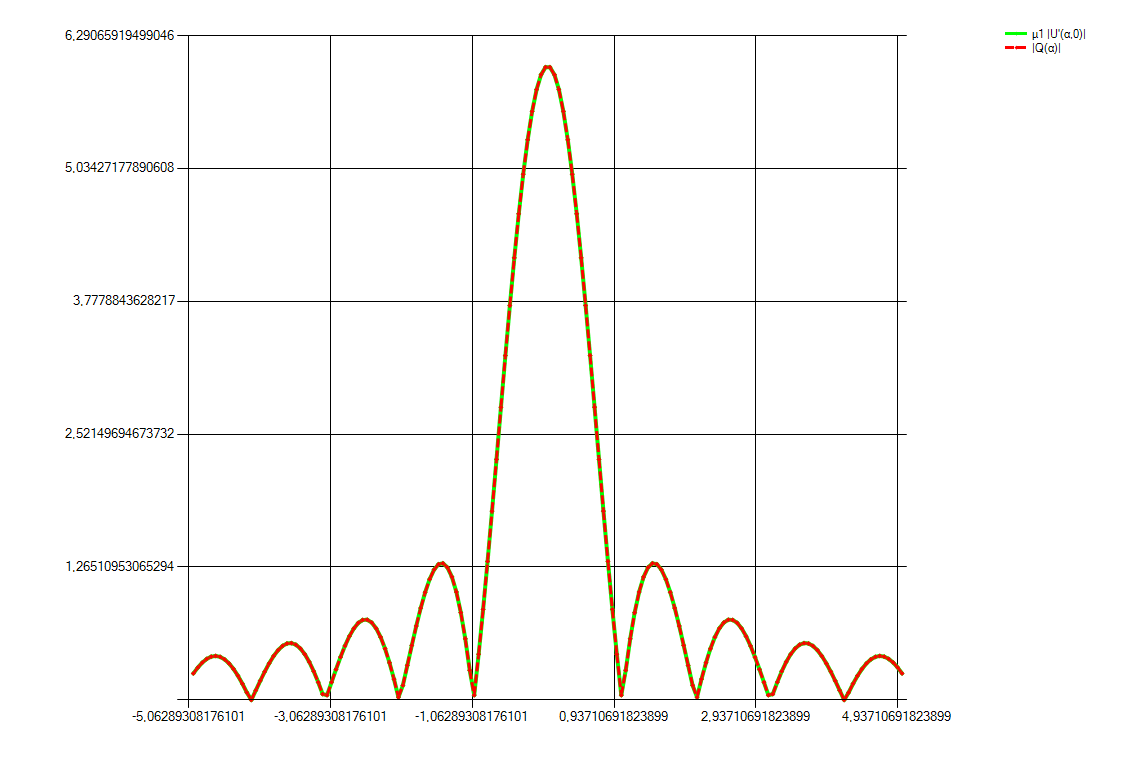
\includegraphics[width=0.7\linewidth]{11.png}
}
\caption{Первое граничное условие в трансформантах}
\label{figCurves}
\end{figure}

\begin{figure}[h!]
\noindent\centering{
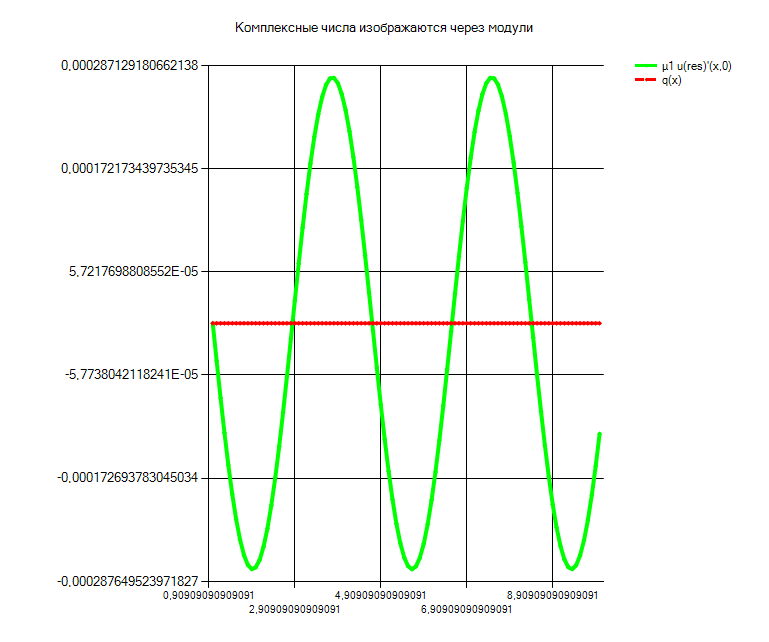
\includegraphics[width=0.7\linewidth]{12.png}
}
\caption{Первое граничное условие после обратного преобразования Фурье}
\label{figCurves}
\end{figure}

Как видно, в трансформантах первое граничное условие выполняется точно (Рис. 2), но обратное преобразование Фурье (подсчёт несобственного интеграла) приводит к приближённому результату (Рис.3) в следствие погрешностей квадратурных формул и ошибок округления. Можно управлять точностью интегрирования для конкретной функции, зная её действительные полюса и совершая их обход при интегрировании. Из практики решения подобных задач известно, что полюса функции $U(\alpha,z)$ совпадают с нулями $\Delta$.

\begin{figure}[h!]
\noindent\centering{
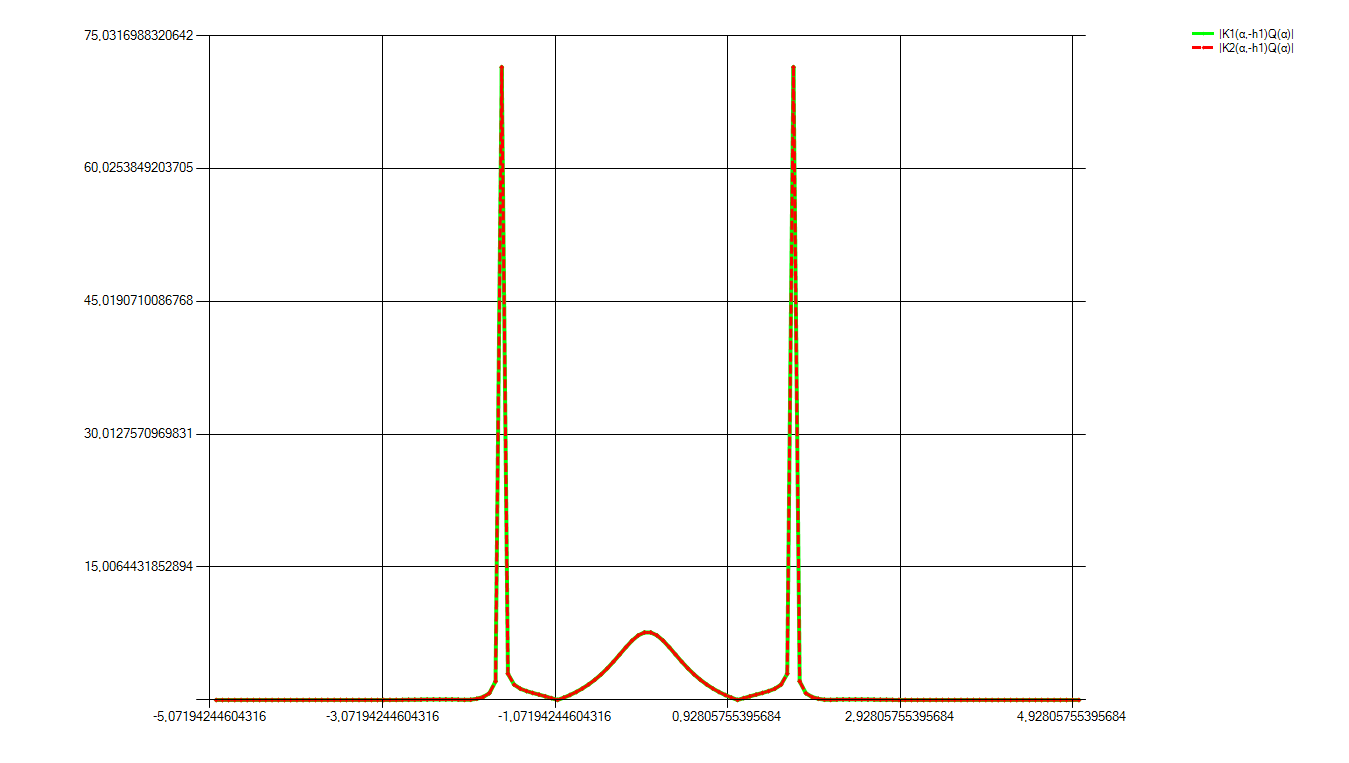
\includegraphics[width=0.9\linewidth]{31.png}
}
\caption{Третье граничное условие в трансформантах}
\label{figCurves}
\end{figure}

\begin{figure}[h!]
\noindent\centering{
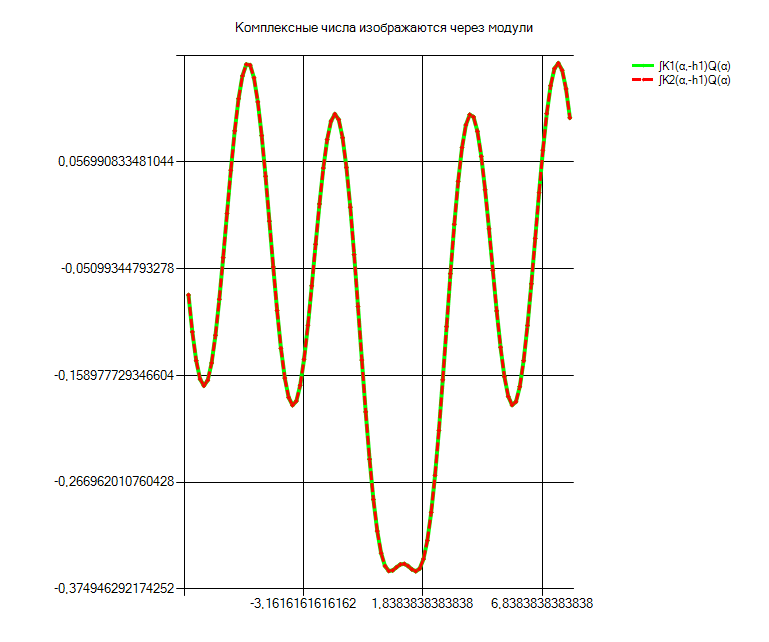
\includegraphics[width=170mm]{32.png}
}
\caption{Третье граничное условие после обратного преобразования Фурье}
\label{figCurves}
\end{figure}


\begin{figure}[h!]
\noindent\centering{
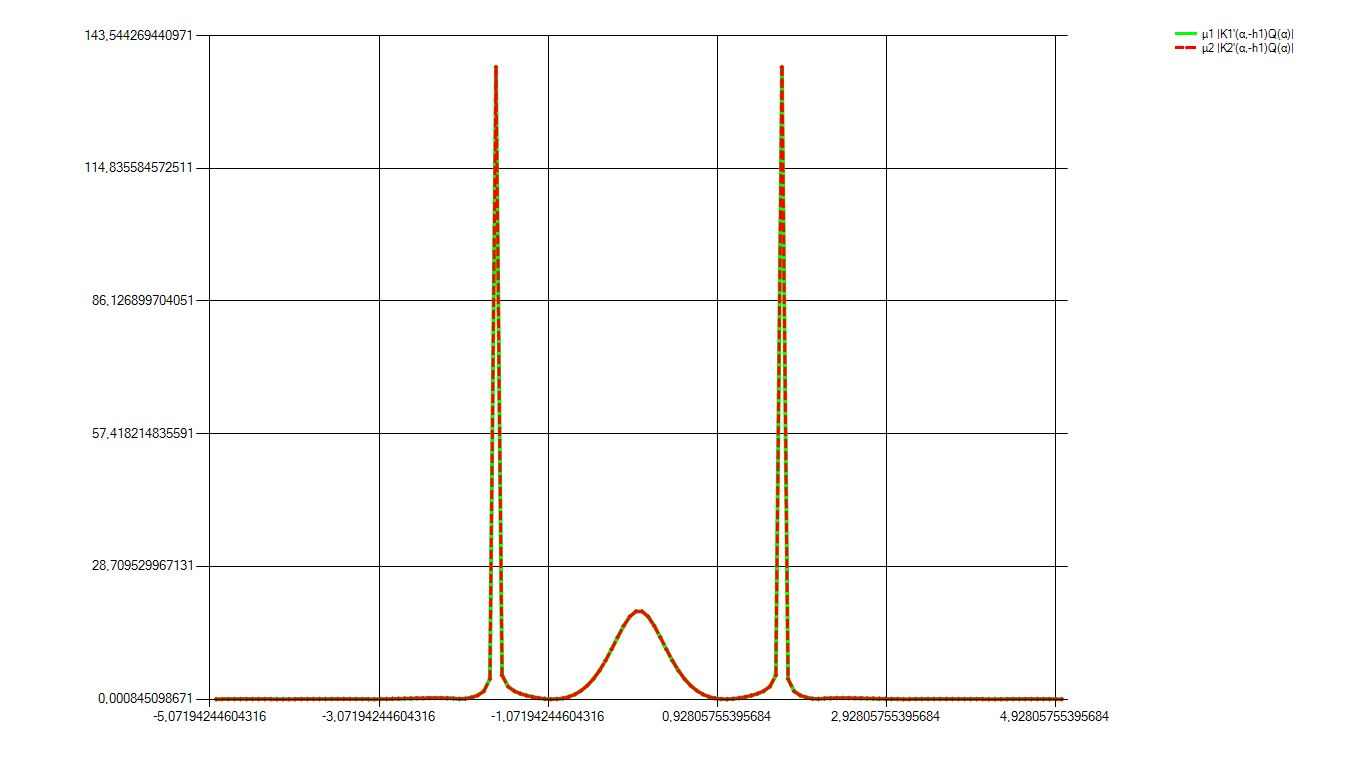
\includegraphics[width=170mm]{41.png}
}
\caption{Четвёртое граничное условие в трансформантах}
\label{figCurves}
\end{figure}

\begin{figure}[h!]
\noindent\centering{
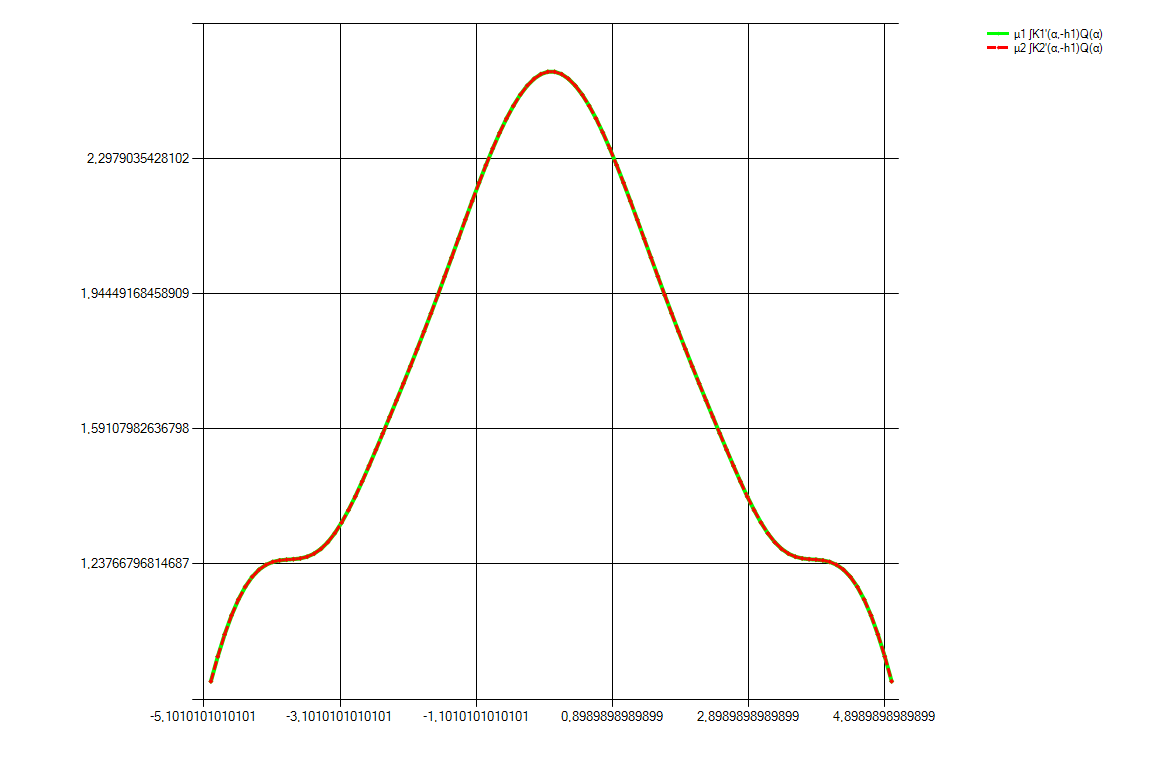
\includegraphics[width=170mm]{42.png}
}
\caption{Четвёртое граничное условие после обратного преобразования Фурье}
\label{figCurves}
\end{figure}

Скачки в трансформантах (Рис. 4, Рис. 6) говорят о том, что вблизи этих скачков находятся полюса функции. Наличие у функции полюсов на некотором множестве становится серьёзной проблемой при интегрировании по этому множеству, поскольку без использования специальных методов и без знания о настоящем положении полюсов численное значение интеграла может существенно отличаться от истинного. А поскольку в конкретном случае искомая функция задана через интеграл, неправильные вычисления способны сильно исказить многие свойства этой функции, в том числе и непрерывность. Эта проблема в данном случае решается следующим образом: по лемме Жордана мы имеем право заменить интеграл
$$u(x,z) =\frac{1}{2\pi} \int^{\infty}_{-\infty} U(\alpha, z) e^{-i \alpha x} d\alpha$$
интегралом
$$u(x,z) =\frac{1}{2\pi} \int_{\Gamma\cup C_R} U(\alpha, z) e^{-i \alpha x} d\alpha \rightarrow\frac{1}{2\pi} \int_{\Gamma} U(\alpha, z) e^{-i \alpha x} d\alpha, R\rightarrow \infty,$$
где $\Gamma$ -- вещественная ось с "изгибами" для обхода полюсов, $C_R$ -- полуокружность с центром в начале координат со стремящимся к бесконечности радиусом; предыдущая формула будет справедлива, если интеграл по этой полуокружности будет стремиться к нулю при увеличении радиуса (лемма Жордана). Отметим, что для выполнения условий излучения Зоммерфельда контур $\Gamma$ должен обходить отрицательные вещественные полюса сверху, положительные -- снизу (Рис. 8).
\begin{figure}[h!]
\noindent\centering{
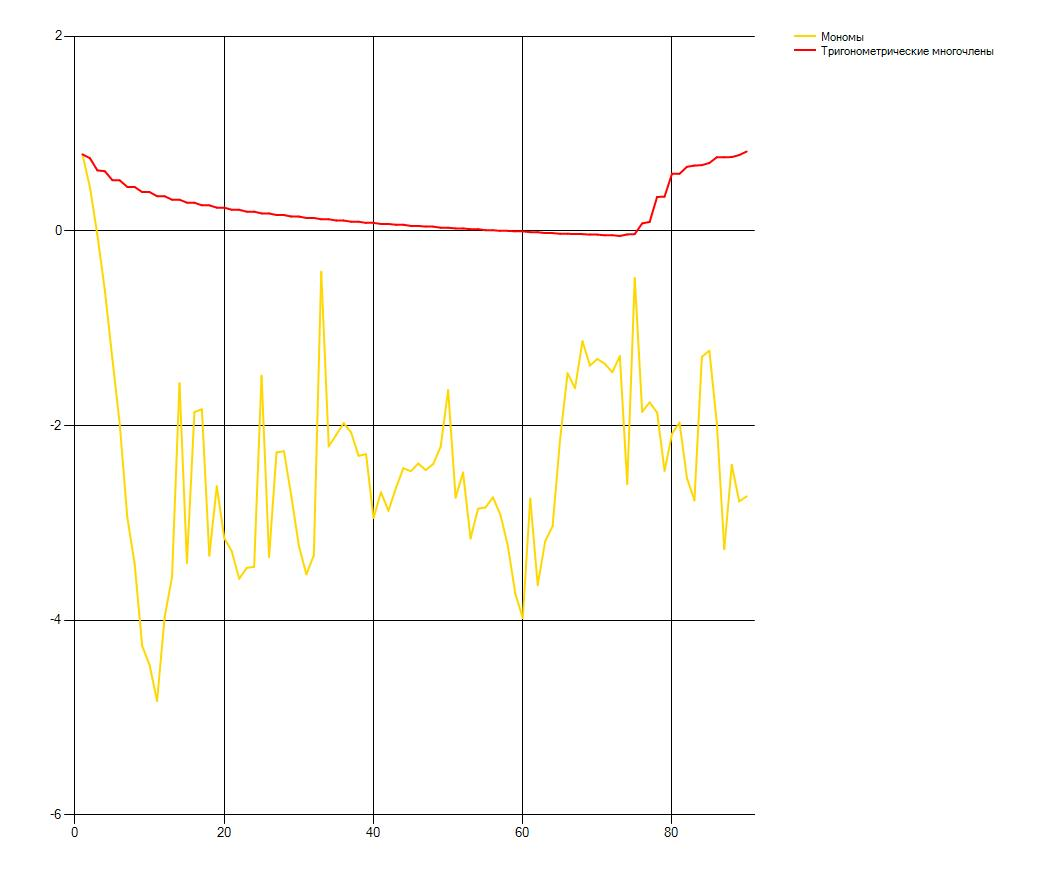
\includegraphics[width=13cm]{5.png}
}
\caption{Обход вещественных полюсов в соответствии с условиями излучения Зоммерфельда}
\label{figCurves}
\end{figure} 


\section{Использование непрерывных радикалов}
Ясно, что сам несобственный интеграл существует только если подынтегральная функция убывает с некоторой скоростью при $z\rightarrow \pm \infty$, поэтому численное интегрирование проводится по конечной кривой $\Gamma$. Кроме того, нет необходимости вычислять интеграл в обе стороны вещественной оси, так как, сэкономив на вычислениях, можно получить тот же результат, вычислив интеграл
$$u(x,z) =\frac{1}{2\pi} \int_{\Gamma'} U(\alpha, z) (e^{-i \alpha x}+e^{i \alpha x}) d\alpha=\frac{1}{\pi}\int_{\Gamma'} U(\alpha, z) \ch (i \alpha x) d\alpha,$$
где $\Gamma'$ -- контур с обходом вещественной полуоси $[0;\infty)$; заметим, что исходная функция $U(\alpha,z)$ чётна по $\alpha$ ввиду того, что аргумент $\alpha$ входит в неё только через суперпозицию в функциях $\sigma_i = \sqrt{\alpha^2-\kappa^2_i}$. Сразу же требуется отметить, что функции $\sigma_i$ должны быть посчитаны особым образом, чтобы сохранять непрерывность. Поясним на примере.

Пусть при подсчёте корней используется стандартная формула из комплексного анализа, то есть в качестве значения $\sigma_i(\alpha)$ выбирается 
$$\sqrt{|\alpha^2-\kappa^2_i|}\exp{\dfrac{i \arg (\alpha^2-\kappa^2_i)}{2}}$$ 
либо
$$\sqrt{|\alpha^2-\kappa^2_i|}\exp\left({\dfrac{i \arg (\alpha^2-\kappa^2_i)}{2}+\pi i}\right);$$
в таком случае будут наблюдаться скачки у искомой функции, например (Рис. 9).
\begin{figure}[h!]
\noindent\centering{
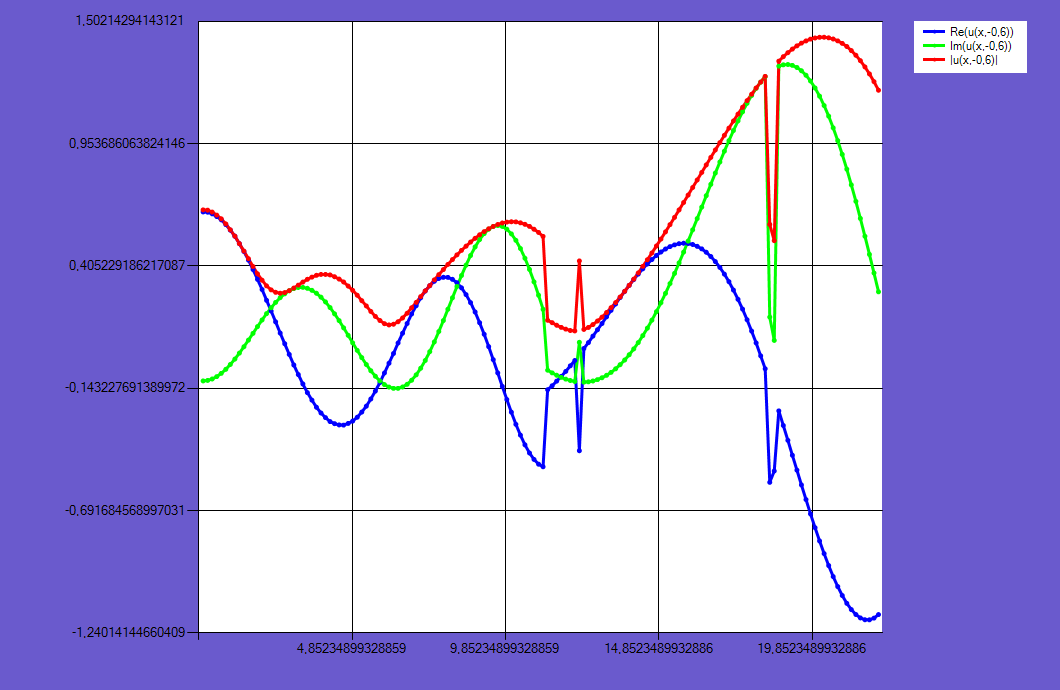
\includegraphics[width=\linewidth]{xbad.png}
}
\caption{График действительной, мнимой части и модуля функции $u(x,-0.6)$ при параметрах: $x \in [0;22], c_2=2, c_1=h_1=h_2=m_1=m_2=\omega=a=1$}
\label{figCurves}
\end{figure}

Из графика видно, что функция имеет несколько локальных скачков, что можно списать на ошибки при интегрировании, однако при $x \approx 11$ (середина графика) наблюдается скачок первого рода (явно неустранимый разрыв), что нельзя оправдывать неточным подсчётом интеграла. Попробуем сперва устранить локальные скачки (из более простого примера на Рис. 10); кривая $\Gamma$, по которой ведётся интегрирование, представляется в виде объединения: $\Gamma=[0;t_0] \cup [t_0;t_0-i t_m] \cup [t_0 - i t_m; t_4 - i t_m] \cup [t_4-i t_m; t_4]\cup [t_4 \cup g_{\Gamma}]$, где $t_0,t_m,t_4,g_{\Gamma}$ -- некоторые действительные числа, выбранные для обхода полюсов подынтегральной функции (будем пока что считать, что все действительные полюса находятся внутри некоторого большого отрезка $[t_0,t_4]$). Как оказывается, скачки значений при интегрировании происходят на отрезке $[t_0 - i t_m; t_4 - i t_m]$; заметим так же, что интегралы по $[t_0;t_0-i t_m]$ и $[t_4-i t_m; t_4]$ равны нулю (Рис. 11).
\begin{figure}[h!]
\noindent\centering{
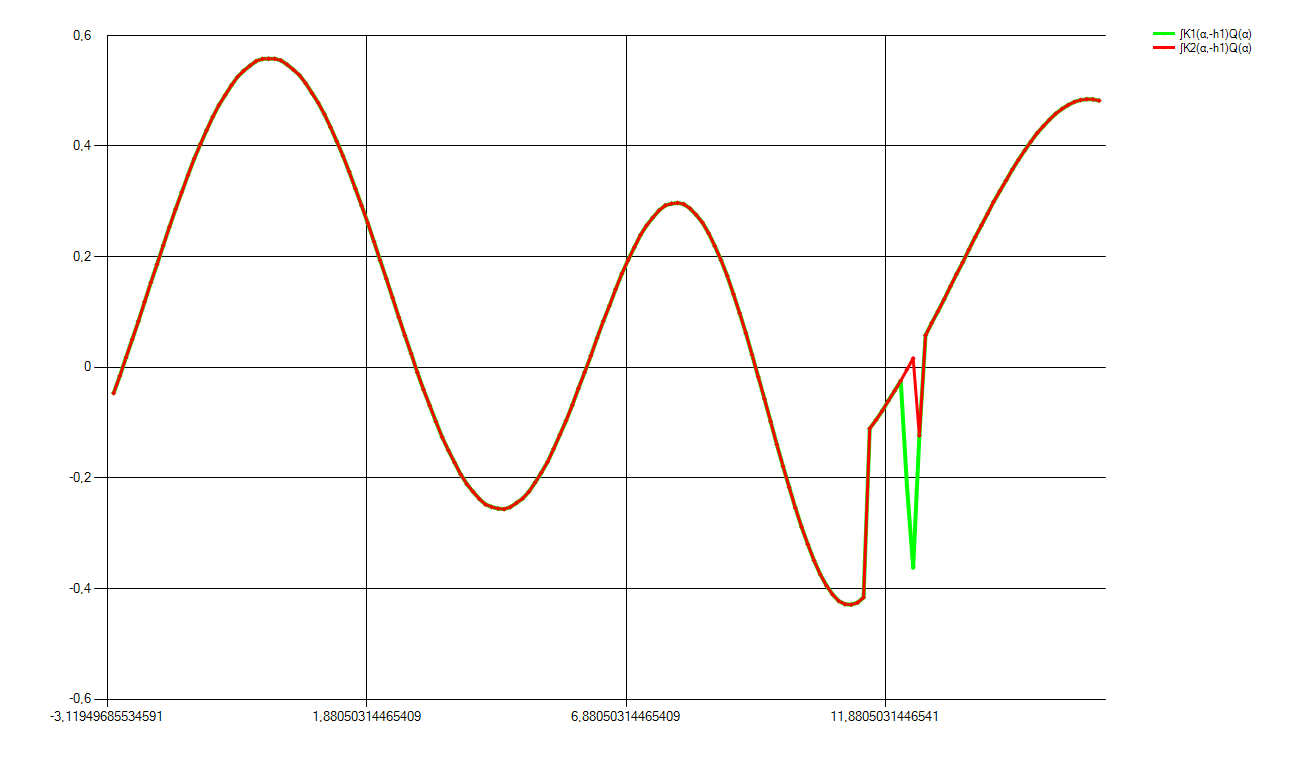
\includegraphics[width=\linewidth]{gr3.png}
}
\caption{Одно из граничных условий с примером разрывной функции}
\label{figCurves}
\end{figure}
\begin{figure}[h!]
\noindent\centering{
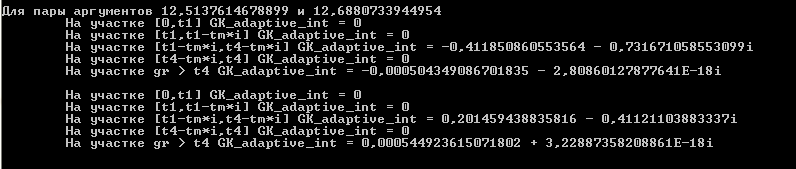
\includegraphics[width=180mm]{otr.png}
}
\caption{На скриншоте показано, что модули функции $\int_{[t_0 - i t_m; t_4 - i t_m]} K_1(\alpha,-h_1)Q(\alpha) d\alpha$ в точках 12.513\dots и 12.688\dots различаются почти в два раза, из-за чего происходит скачок. Этот скачок можно увидеть у красной кривой на следующем рисунке}
\label{figCurves}
\end{figure}



Пусть $F(\alpha,x,z)=K_2(\alpha,z)Q(\alpha)\ch(i\alpha x)$, то есть $F$ -- подынтегральная функция для расчёта $u$; изобразим действительную и мнимую часть $F$, например, на отрезке $\alpha \in [0.2i;15-0.2i]$ при $x=2, z=-1$ (Рис. 12). Не вызывает сомнений факт разрывности функции $F$, что никак не связано с интегрированием, поскольку $F$ -- лишь суперпозиция трансформант. 
\begin{figure}[h!]
\noindent\centering{
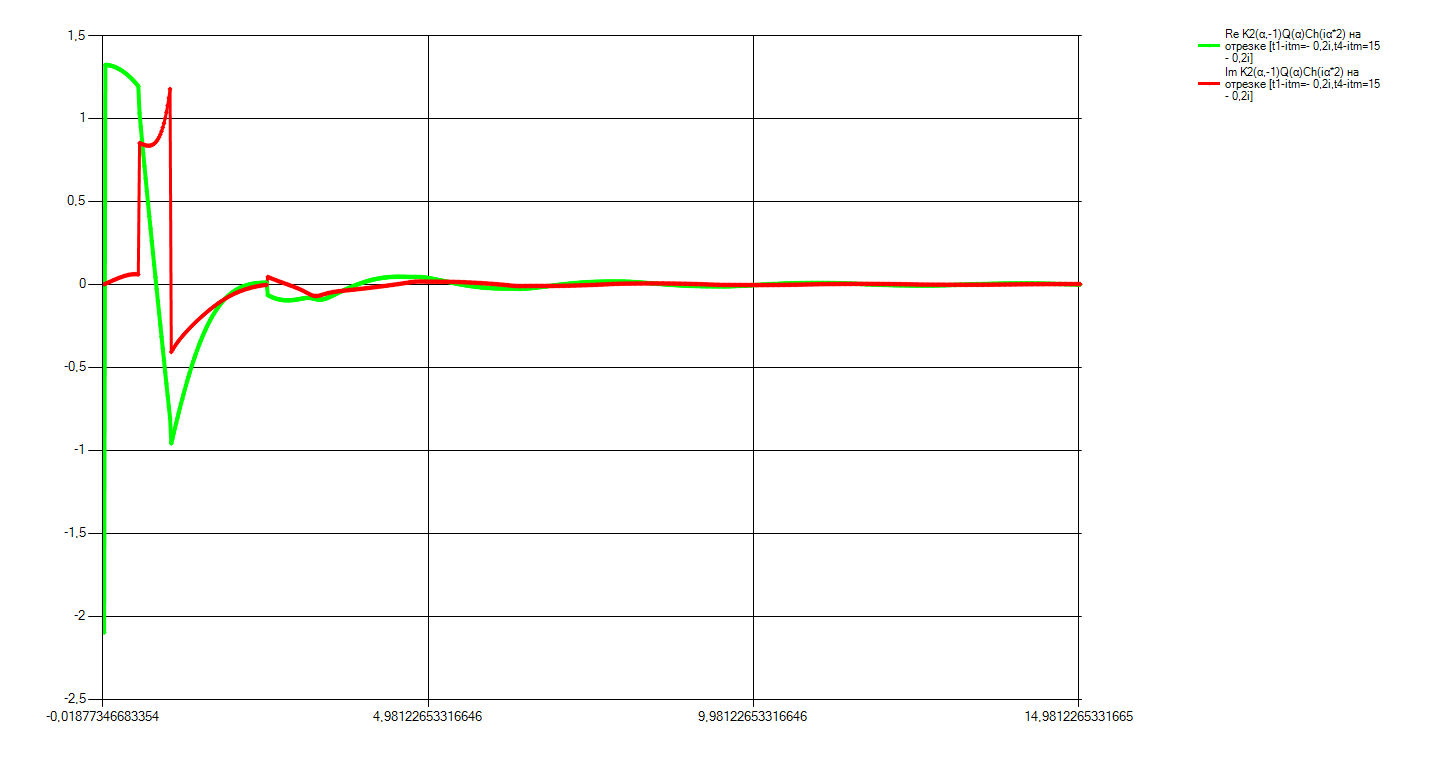
\includegraphics[width=\linewidth]{F.png}
}
\caption{Действительная и мнимая часть $F(\alpha,2,-1), \alpha \in [0.2i;15-0.2i]$}
\label{figCurves}
\end{figure}

Так как функции $\sin z, e^z, \frac{1}{z}$ аналитичны во всей комплексной плоскости (возможно, без одной точки), то разрывность нужно искать в радикалах. И действительно, функция $\sigma_1=\sqrt{\alpha^2-\kappa^2_1}$ имеет разрывы на том же отрезке (Рис. 13).
\begin{figure}[h!]
\noindent\centering{
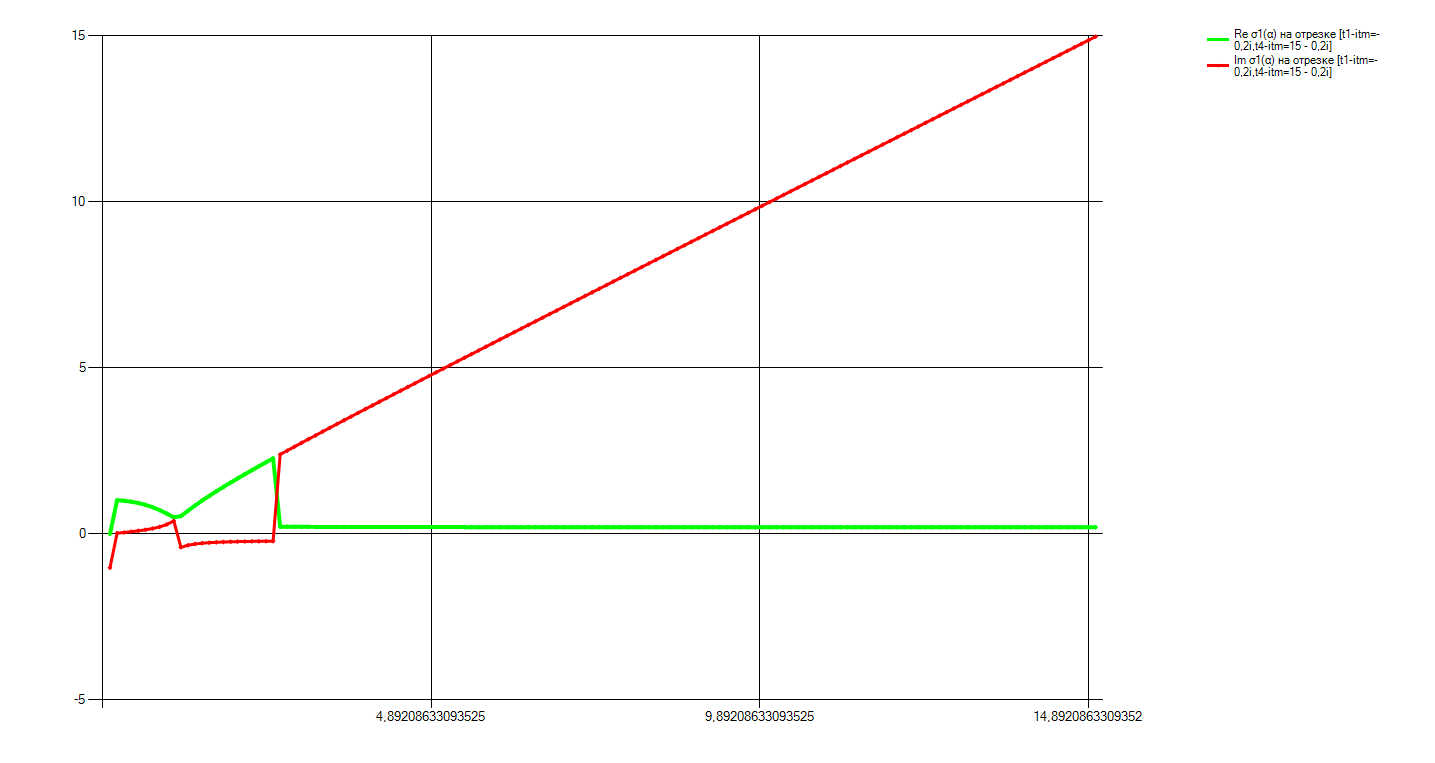
\includegraphics[width=\linewidth]{sigma1.png}
}
\caption{Действительная и мнимая часть $\sigma_1 (\alpha), \alpha \in [0.2i;15-0.2i]$}
\label{figCurves}
\end{figure}

Разрывы радикала связаны с переходом на другую ветвь при $|\alpha|=|\kappa_i|$, причём результаты перехода сложно контролировать, особенно если функция поиска корня "зашита" внутри языка программирования и неизвестна пользователю. Сам разрыв связан с неоднозначным заданием комплексного числа в полярных координатах. Например, пусть $a$ и $b$ - некоторые действительные числа, причём $b>a$; тогда для комплексного числа $a-b$ верно, что $\arg(a-b)=\pi$, но в то же время $\arg(a-b)=-\pi$; пока мы работаем с числом $a-b$, оба аргумента считаются равнозначными, однако уже при извлечении квадратного корня по одной из приведённых ранее формул получаются два комплексных числа с аргументами $\frac{\pi}{2}$ и $-\frac{\pi}{2}$. Независимо от того, как именно задается разрез радикала (через отрицательную действительную полуось или иначе), погрешности округления способствуют скачкам на другие ветви. Чтобы функция радикала $\sigma(\alpha)=\sqrt{\alpha^2-\kappa^2}$ оставалась непрерывной, её нужно задавать с условиями, учитывая конкретные значения $\alpha$ и $\kappa$; задать можно, к примеру, следующим образом:
\begin{enumerate}
    \item пусть sqrt$(z)=|z|e^{i\arg z},-\pi < \arg z \leq \pi$ и пусть $r=|\alpha^2-\kappa^2|$
    \item в частности, если $\alpha$ -- действительное число ($\Im \alpha=0$)
    \begin{enumerate}
        \item при $|\alpha|\geq\kappa\  \sigma = \sqrt{r}$ 
        \item при $|\alpha|<\kappa\  \sigma = -i\sqrt{r}$ 
    \end{enumerate}
    \item в общем случае 
    \begin{enumerate}
    \item если $|\alpha|>|\kappa|$, то $\sigma=$ sqrt$(\alpha^2-\kappa^2)$
        \item если $\mathrm{Re} \alpha \ \mathrm{Im} \alpha >0$, то $\sigma=i$ sqrt$(\kappa^2-\alpha^2)$
        \item иначе $\sigma=-i$ sqrt$(\kappa^2-\alpha^2)$
    \end{enumerate}
\end{enumerate}

Если считать радикалы таким способом, то радикал станет непрерывным; предыдущие графики (Рис. 12, Рис. 13) примут вид (Рис. 14, Рис. 15).
\begin{figure}[h!]
\noindent\centering{
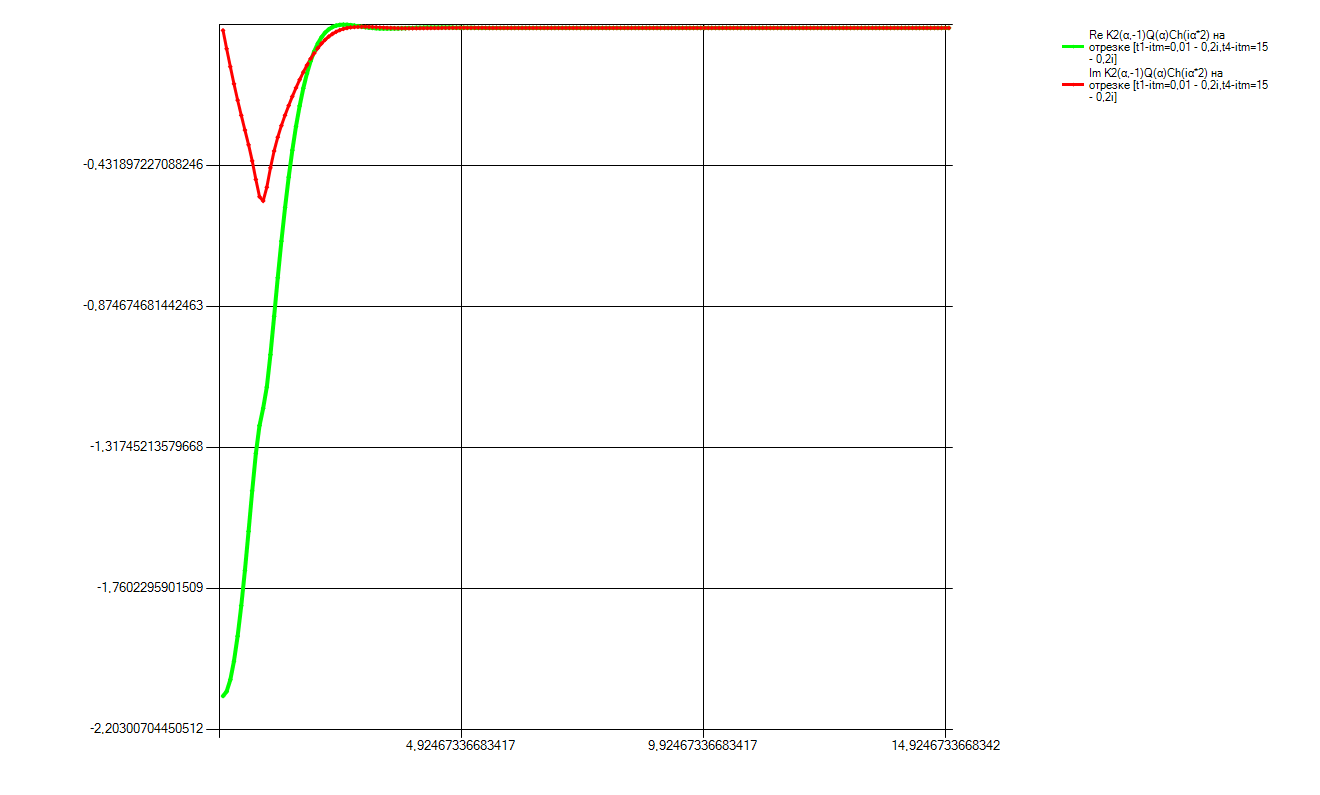
\includegraphics[width=\linewidth]{F2.png}
}
\caption{Действительная и мнимая часть $F(\alpha,2,-1)$}
\label{figCurves}
\end{figure}

\begin{figure}[h!]
\noindent\centering{
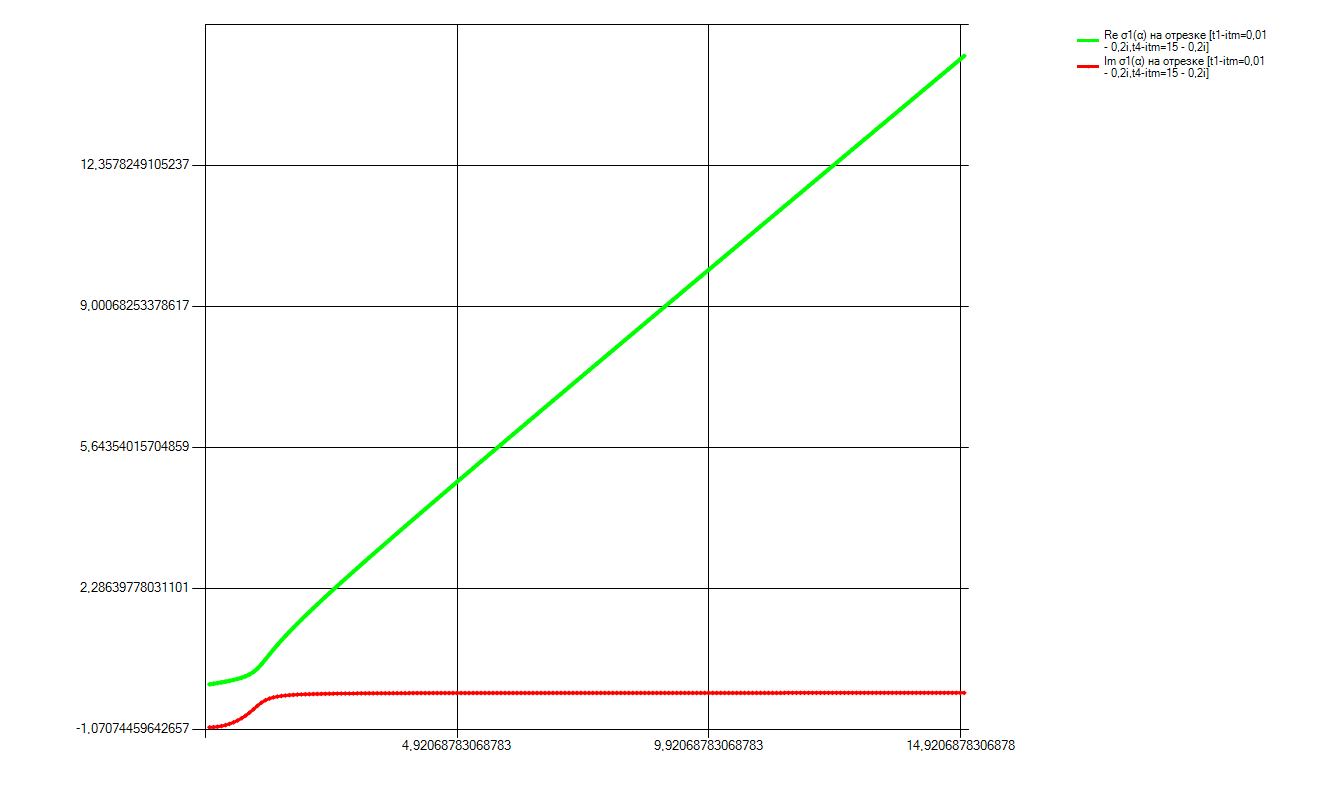
\includegraphics[width=\linewidth]{sigma1n.png}
}
\caption{Действительная и мнимая часть $\sigma_1 (\alpha)$}
\label{figCurves}
\end{figure}


\newpage
\section{Дисперсионные кривые}
При вычислении интеграла
$$u(x,z) =\frac{1}{2\pi} \int_{\Gamma'} U(\alpha, z) (e^{-i \alpha x}+e^{i \alpha x}) d\alpha=\frac{1}{\pi}\int_{\Gamma'} U(\alpha, z) \ch (i \alpha x) d\alpha,$$
прямым способом либо с помощью вычетов, как уже было сказано, требуется знать некоторую информацию о вычетах подынтегральной функции на действительной оси; в первом случае это -- отрезки вне которых вычетов нет; во втором -- конкретное расположение вычетов. Эти данные необходимо получить до подсчёта конкретных интегралов, дабы сэкономить ресурсы при вычислении интегралов при одинаковых параметрах. Известно, что для задач, подобных решаемой, вычеты подынтегральной функции совпадают с нулями $\Delta(\alpha)$, в конкретном случае $ \Delta(\alpha)=\E{-\s{1}}{h_1}(\m{2}\s{2}\sh(\s{2}(h-h_1))-\m{1}\s{1}\ch(\s{2}(h-h_1)))+\E{\s{1}}{h_1}(\m{1}\s{1}\ch(\s{2}(h-h_1))+\m{2}\s{2}\sh(\s{2}(h-h_1)))$. 

Обозначив за $\zeta_\omega$ такие $\alpha$, при которых справедливо уравнение $\Delta(\alpha,\omega)=0$, получим неявные функции $\zeta(\omega), \omega(\zeta)$, задаваемые этим уравнением. Графическое представление указанных зависимостей называют дисперсионными кривыми. График дисперсионных кривых позволяет, в частности, локализовать вычеты подынтегральной функции на фиксированном отрезке, что требуется для задания параметров численного интегрирования.
К примеру, из следующих графиков (Рис. 16, Рис. 17) видно, что для задачи с фиксированными параметрами $c_1=h_1=h_2=\mu_1=1, c_2=1.4, \mu_2=2$ при частоте, допустим, $\omega=5$ (частота откладывается по действительной оси), функция $U(\alpha,z)$ ($z$ считаем за параметр) имеет три действительных полюса на положительной полуоси, расположенных примерно на отрезке  $[2.7;5]$, поэтому при подсчёте несобственного интеграла при таких параметрах контур интегрирования следует отклонить от вещественной оси примерно на этом отрезке; при отклонении контура можно брать отрезок и намного больше, однако в этом случае увеличивается риск попасть на комплексные полюса и получить неправильный интеграл.

\begin{figure}[h!]
\noindent\centering{
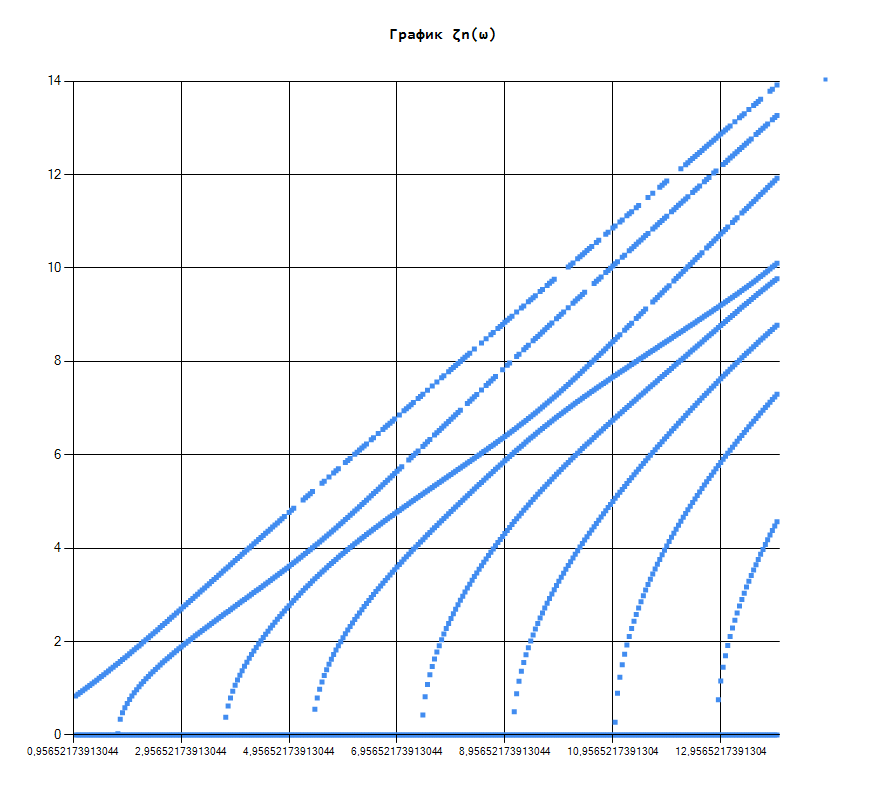
\includegraphics[width=0.6\linewidth]{zn.png}
}
\caption{Кривые $\zeta_n(\omega), \omega \in [1,14]$, при фиксированных параметрах $c_1=h_1=h_2=\mu_1=1,c_2=1.4,\mu_2=2$}
\label{figCurves}
\end{figure}

\begin{figure}[h!]
\noindent\centering{
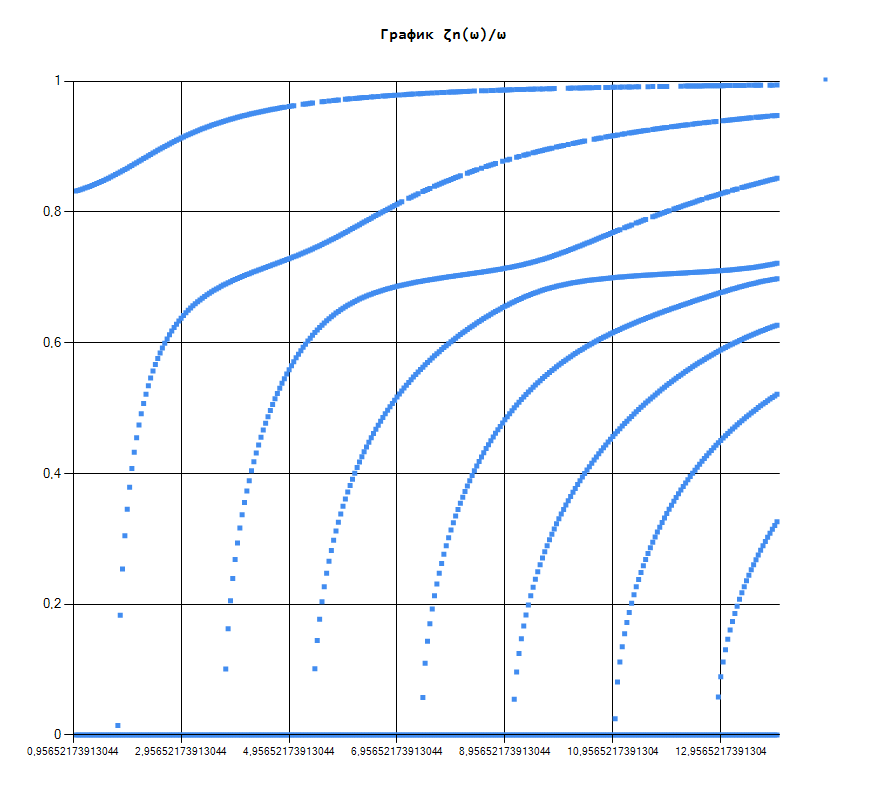
\includegraphics[width=16cm]{sn.png}
}
\caption{Кривые $s_n(\omega)=\dfrac{\zeta_n(\omega)}{\omega}, \omega \in [1,14]$, при фиксированных параметрах $c_1=h_1=h_2=\mu_1=1,c_2=1.4,\mu_2=2$}
\label{figCurves}
\end{figure}

{\bf Замечание.} При поиске корней функции $\Delta$ требуется добиться баланса между шагом поиска, допустимой точностью и максимальным числом итераций (обозначим за $\hbar, \varepsilon, n$ соответственно): 
при слишком маленьком $\hbar$ поиск будет слишком долгим, а при несоразмерных $\varepsilon$ и $n$ алгоритм может пропустить корень, так как число шагов не позволило дойти до нужной точности и добиться результата;
с другой стороны, при большом $\hbar$ также могут пропускаться корни, если на некотором отрезке длины $\hbar$ их содержалось несколько, а большое $n$ при малом $\varepsilon$ заметно удлиняется поиск, так как с приближением к корню может замедляться сходимость.

С учётом сказанного, перед вычислением интеграла требуется не просто отыскать полюса, но, построив несколько графиков дисперсионных кривых, определиться с параметрами поиска: при любой частоте $\omega$ полюсов должно быть найдено столько же, сколько и на соседних частотах, если только при этой частоте не образуется новая волна; дисперсионные кривые в таком случае должны быть визуально без пропущенных точек.
Практика показывает, что для достижения оптимального результата требуется варьировать точность $\varepsilon$ в сторону увеличения. Например, в предыдущих графиках использовались параметры поиска $\hbar=10^{-3}, \varepsilon=10^{-7}, n=20$, причём заметны пропуски точек, особенно у самой верхней кривой; если зафиксировать параметры $\hbar = 10^{-4}, n=1000$, это безрезультатно увеличит время поиска в десяток раз; но если указать $\varepsilon = 10^{-3}$, этого окажется достаточно (Рис. 18).

\begin{figure}[h!]
\noindent\centering{
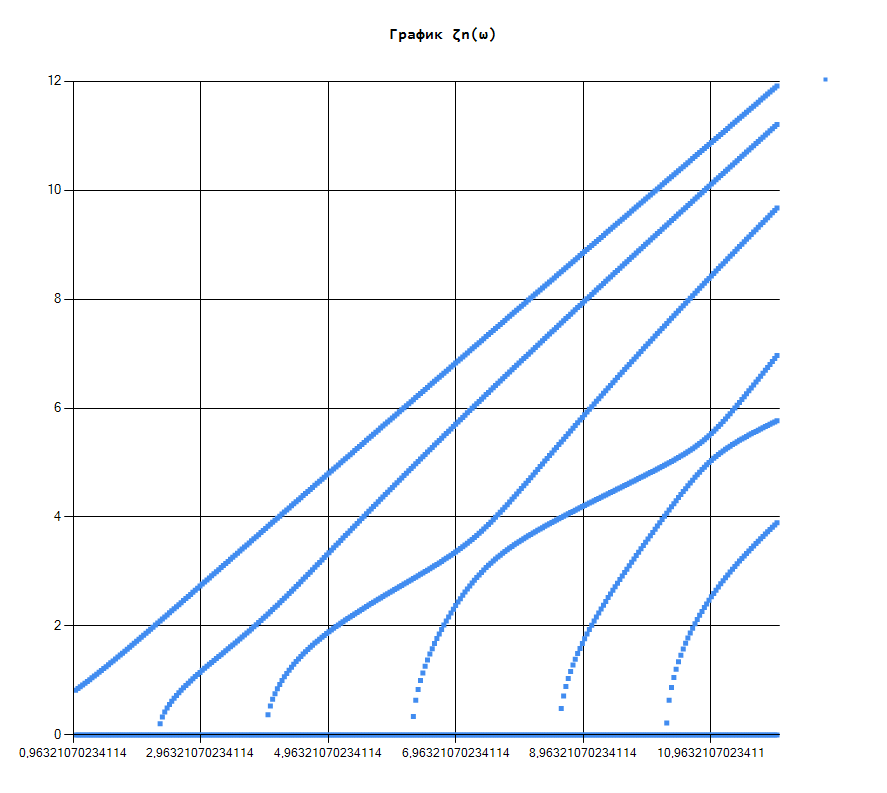
\includegraphics[width=0.95\linewidth]{znnew.png}
}
\caption{Кривые $\zeta_n(\omega), \omega \in [1,14]$, при фиксированных параметрах $c_1=h_1=h_2=\mu_1=1,c_2=1.4,\mu_2=2$ и $\varepsilon = 10^{-3}$}
\label{figCurves} 
\end{figure}

\section{Дополнительные свойства найденного решения}
В этом разделе представлены другие графики, характеризующие поведение функции $u(x,z)$.

\begin{figure}[h!]
\noindent\centering{
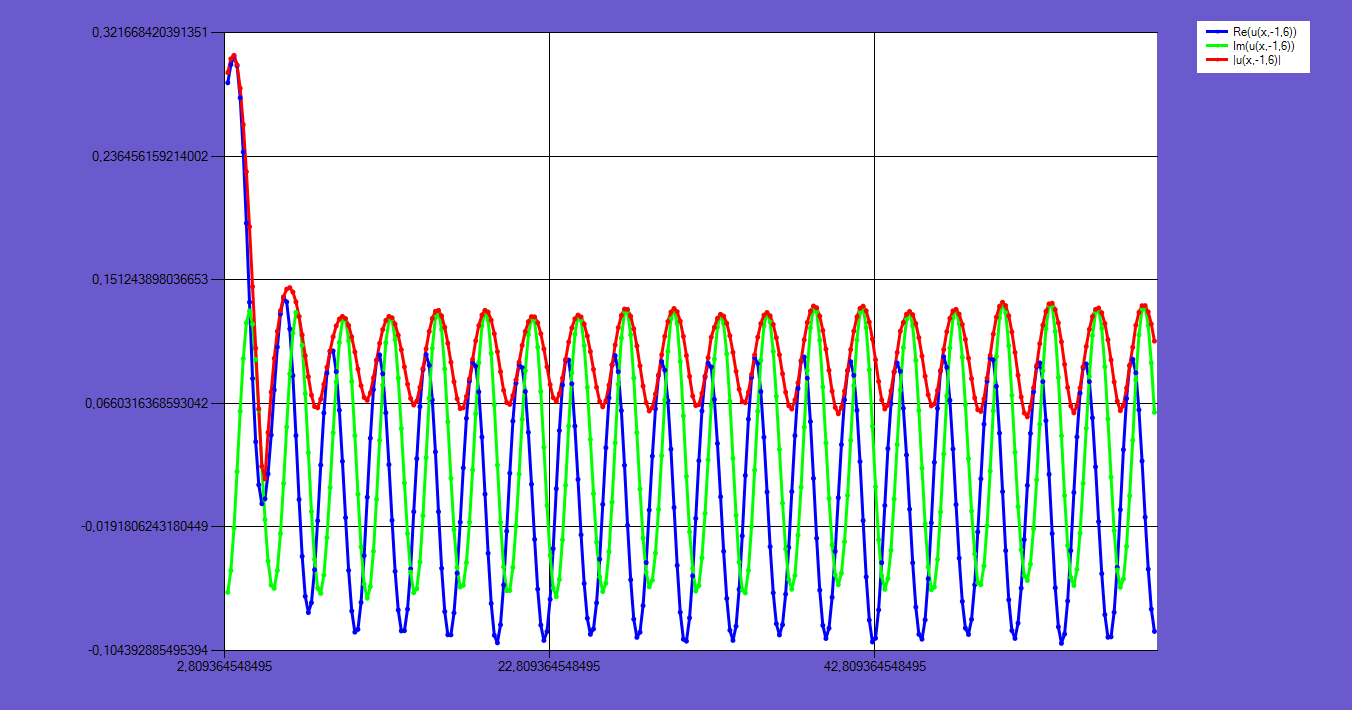
\includegraphics[width=0.95\linewidth]{101.png}
}
\caption{График действительной, мнимой частей и модуля $u(x,z)$ при $z=-1.6, x \in [3;60], c_1=h_1=h_2=x_0=\mu_1=1, c_2=2,\mu_2=1.3,\omega=4$, посчитанных прямым интегрированием}
\label{figCurves}
\end{figure}

\begin{figure}[h!]
\noindent\centering{
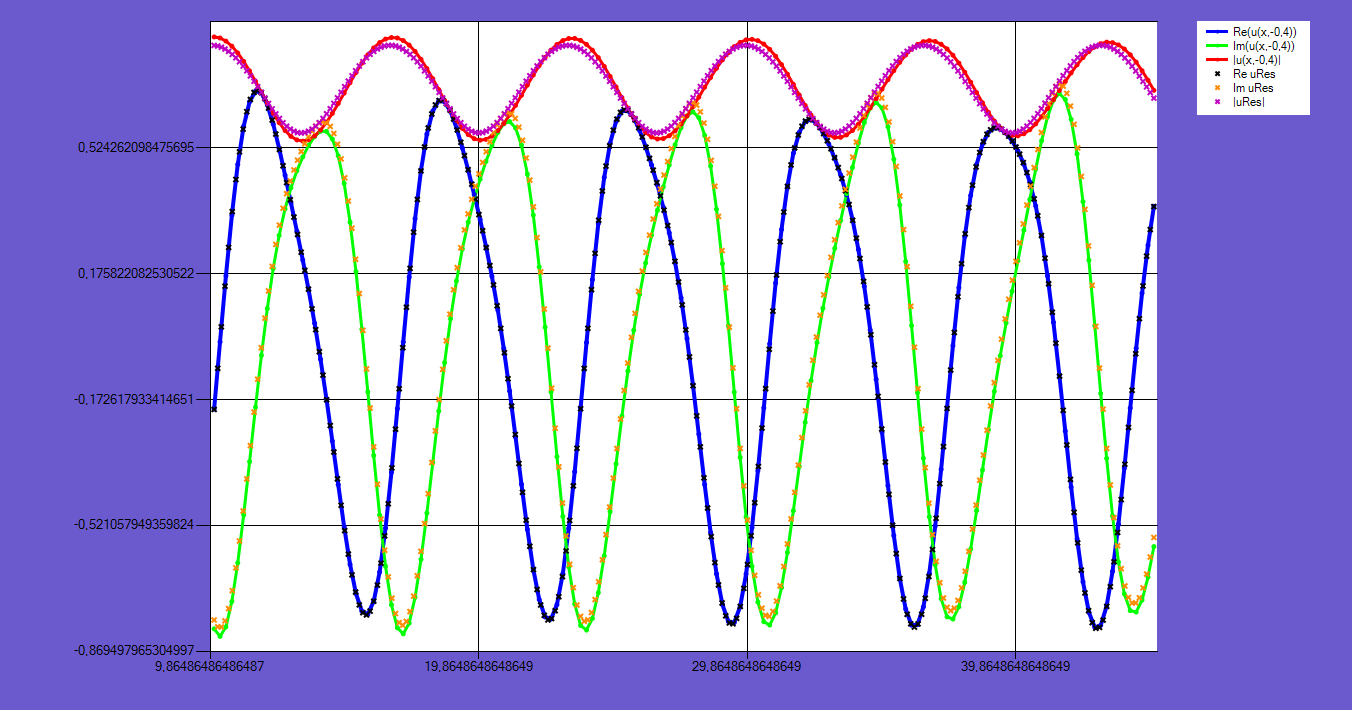
\includegraphics[width=0.95\linewidth]{102.png}
}
\caption{График действительной, мнимой частей и модуля $u(x,z)$ при $z=-0.4, x \in [10;45], c_1=h_1=h_2=\mu_1=1, c_2=1.2,\mu_2=1.1,\omega=2$, посчитанных прямым интегрированием и через вычеты}
\label{figCurves}
\end{figure}

\begin{figure}[h!]
\noindent\centering{
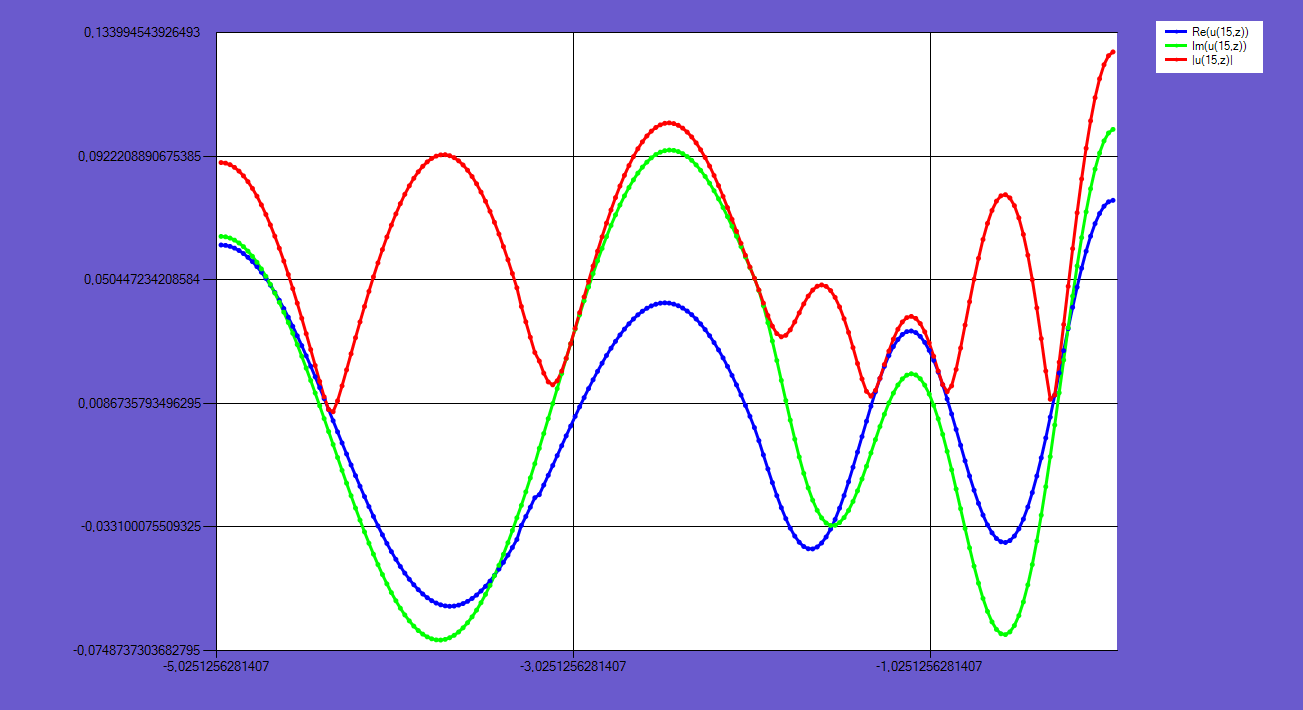
\includegraphics[width=0.95\linewidth]{103.png}
}
\caption{График действительной, мнимой частей и модуля $u(x,z)$ при $x=15, z \in [-5;0], c_1=\mu_1=1, c_2=h_1=2, h_2=3, \mu_2=1.2$, посчитанных прямым интегрированием}
\label{figCurves}
\end{figure}

\begin{figure}[h!]
\noindent\centering{
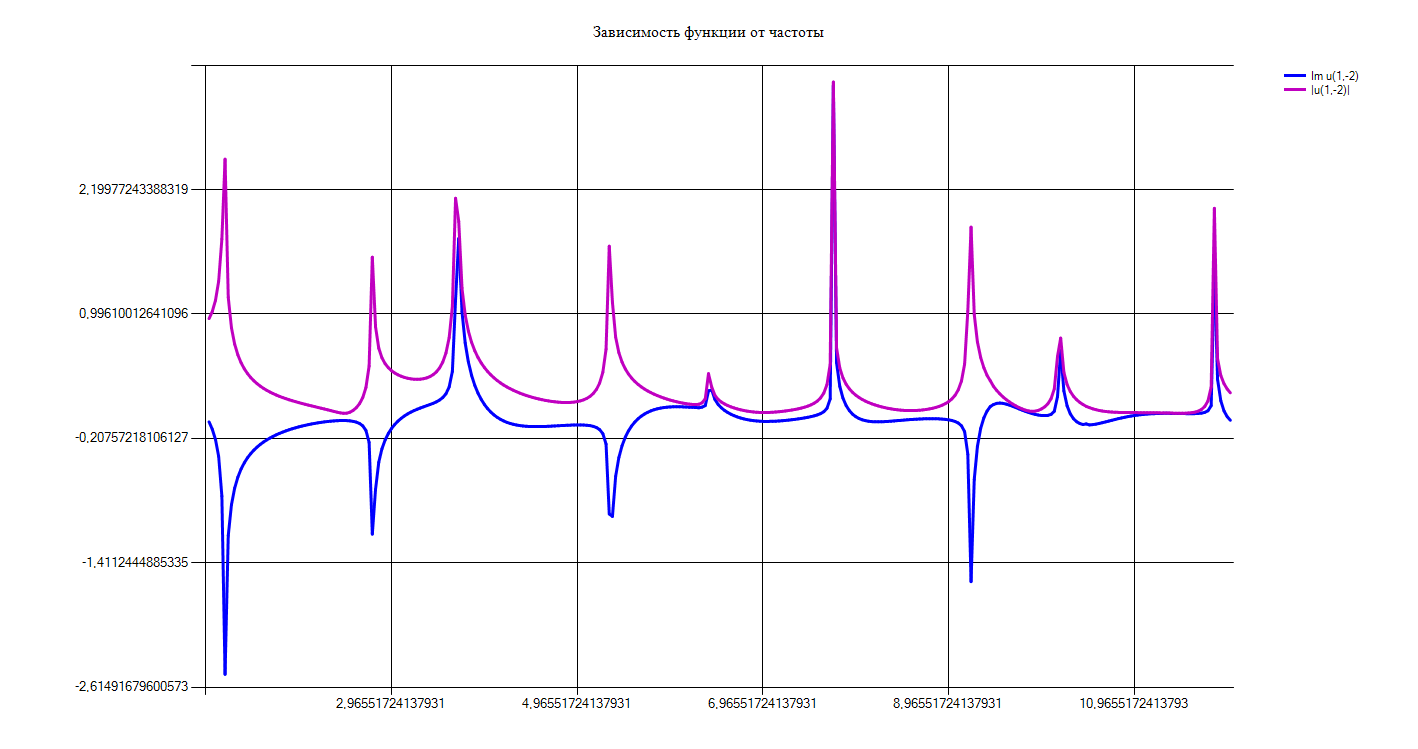
\includegraphics[width=\linewidth]{1104.png}
}
            \caption{График зависимости мнимой части и модуля $u(x,z)$ от частоты при $x=1, z=-2, c_1=\mu_1=h_1=1, c_2=1.4, h_2=2, \mu_2=0.5, \omega \in [1;12]$}
            \label{figCurves}
            \end{figure}  
            
            \begin{figure}[h!]
                \noindent\centering{
                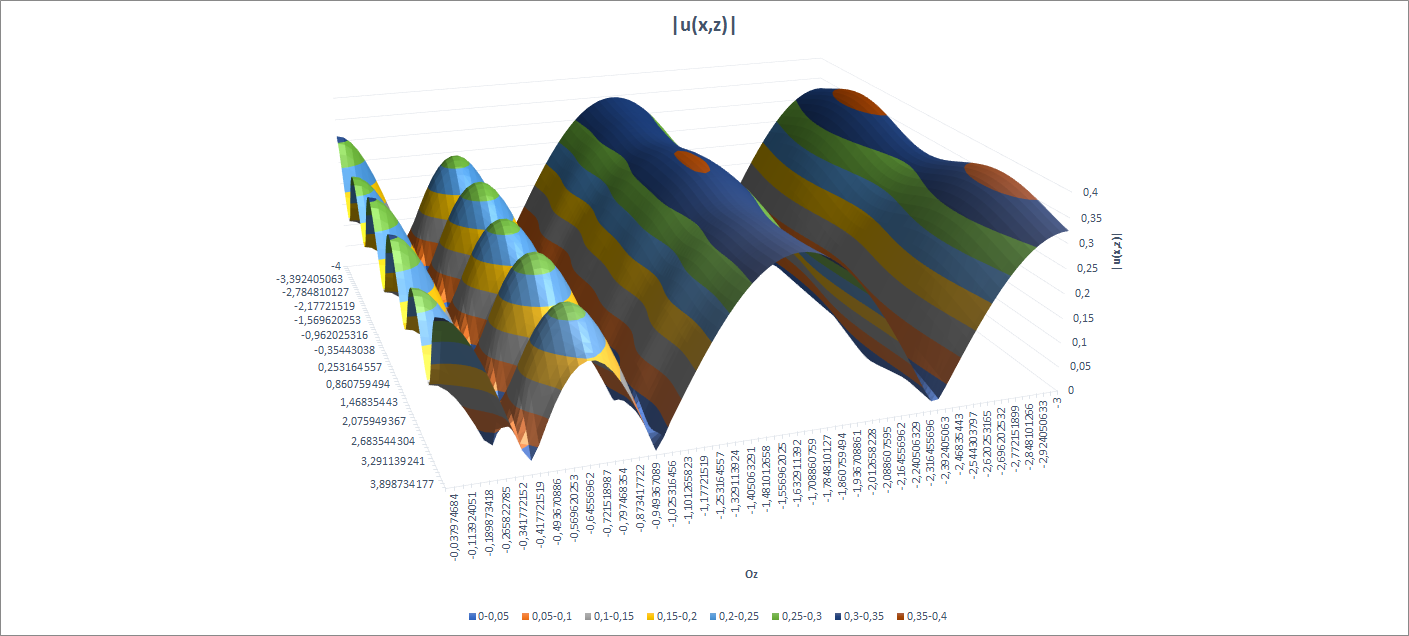
\includegraphics[width=0.95\linewidth]{105.png}
                }
                \caption{График модуля $u(x,z)$ при $x \in [-4;4], z \in [-3;0], c_1=\mu_1=h_1=1, c_2=h_2=2, \mu_2=1.4, \omega =5$}
                \label{figCurves}
                \end{figure}

    \begin{figure}[h!]
    \noindent\centering{
    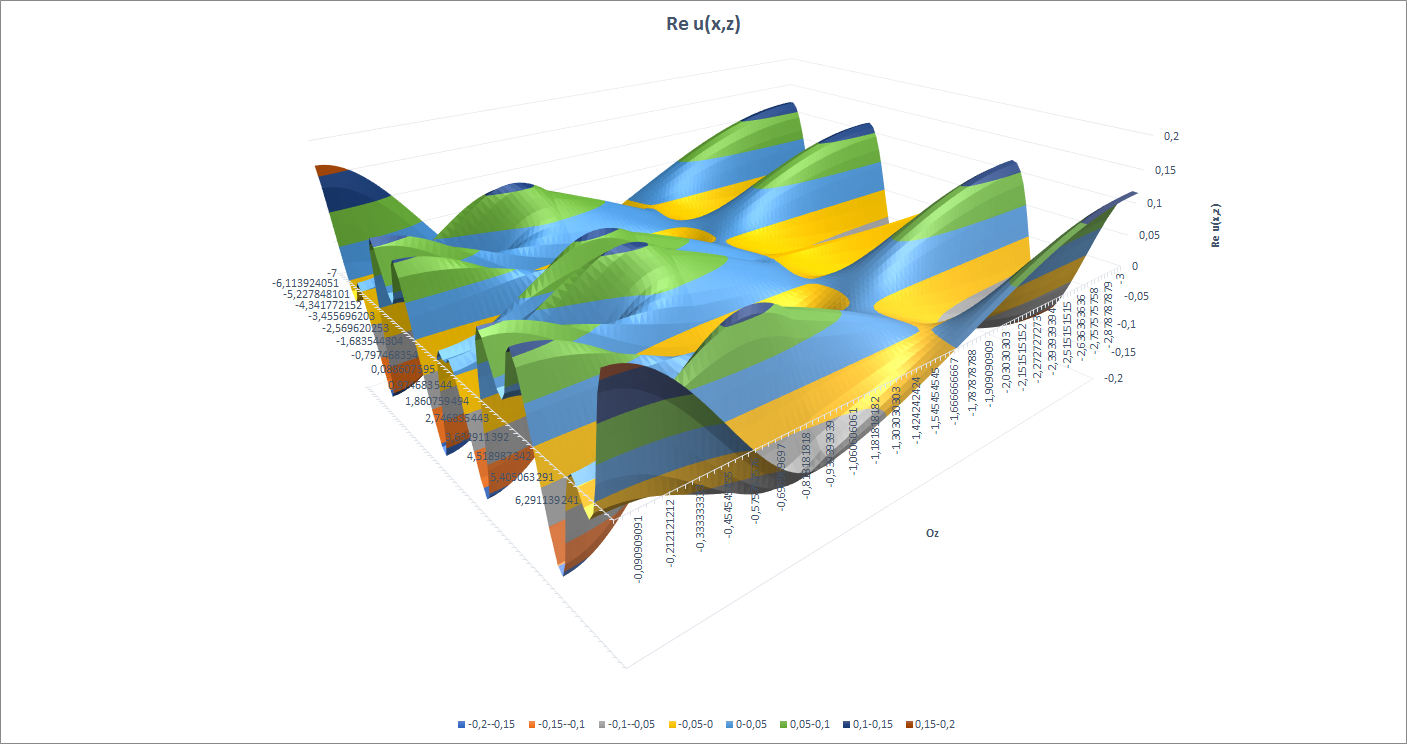
\includegraphics[width=0.95\linewidth]{106.png}
  }
    \caption{График действительной части $u(x,z)$ при $x \in [-7;7], z \in [-3;0], c_1=\mu_1=h_1=1, c_2=h_2=\mu_2=2, \omega =4$}
    \label{figCurves}
    \end{figure}  

    \begin{figure}[h!]
        \noindent\centering{
        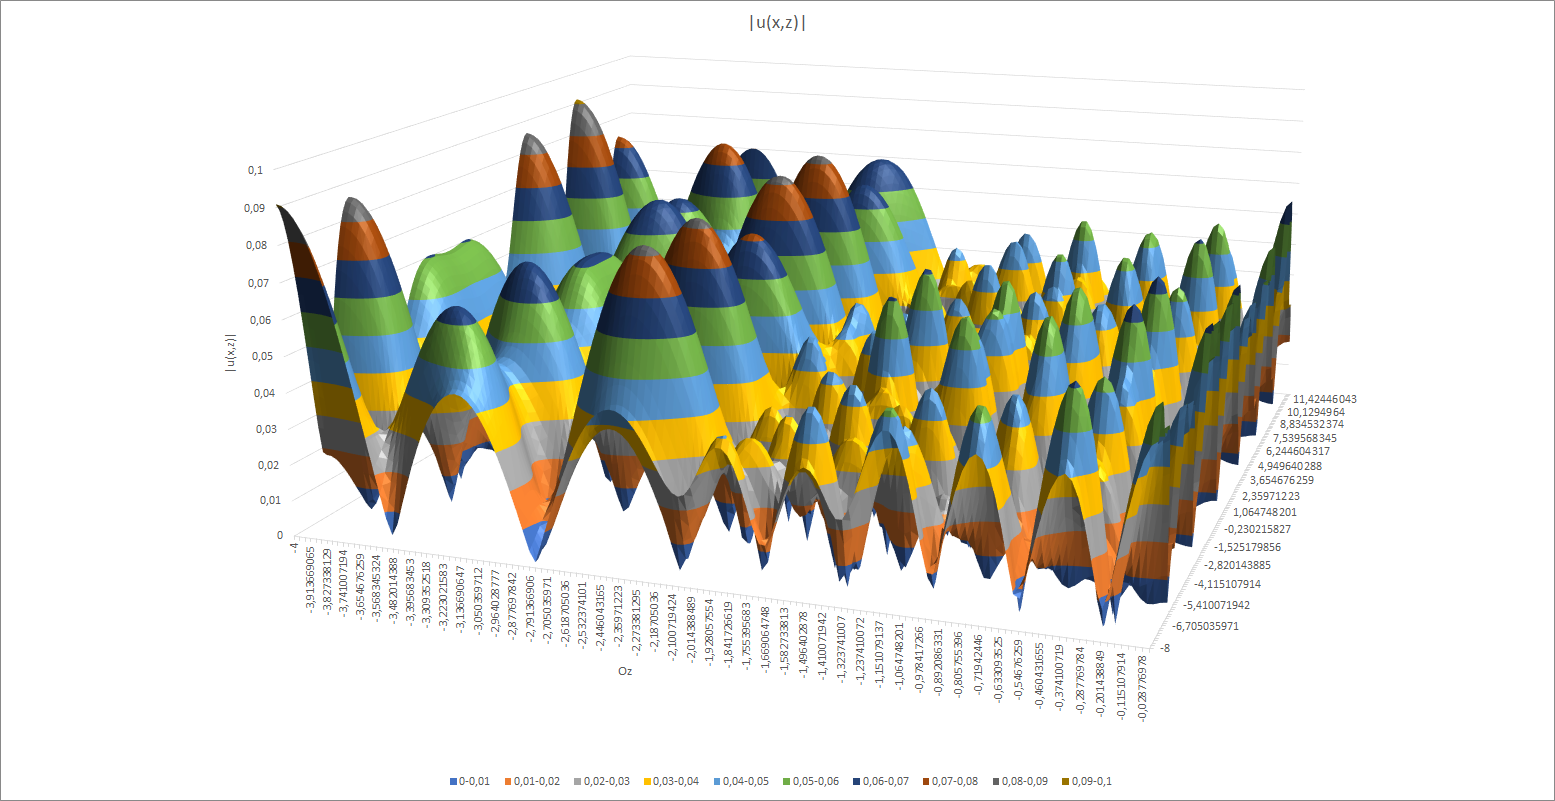
\includegraphics[width=0.95\linewidth]{107.png}
      }
        \caption{График модуля $u(x,z)$ при $x \in [-8;12], z \in [-4;0], c_1=\mu_1=1, c_2=h_1=h_2=2, \omega =9, \mu_2=1.1$}
        \label{figCurves}
        \end{figure} 

        \begin{figure}[h!]
            \noindent\centering{
            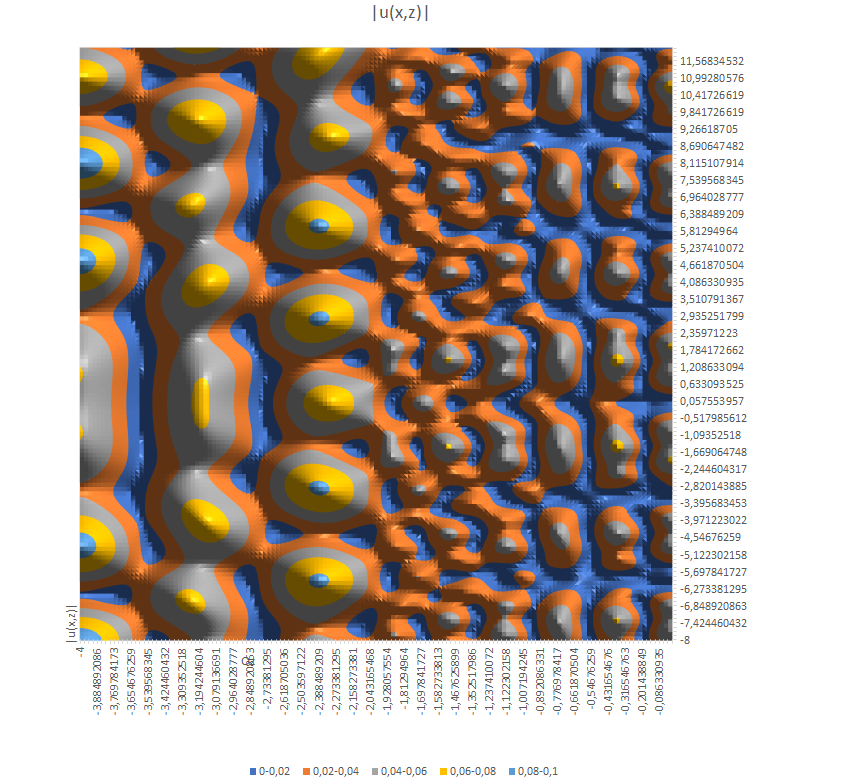
\includegraphics[width=0.95\linewidth]{108.png}
          }
            \caption{Вид сверху на предыдущий график (линии уровня)}
            \label{figCurves}
            \end{figure} 
    
\begin{figure}[h!]
\noindent\centering{
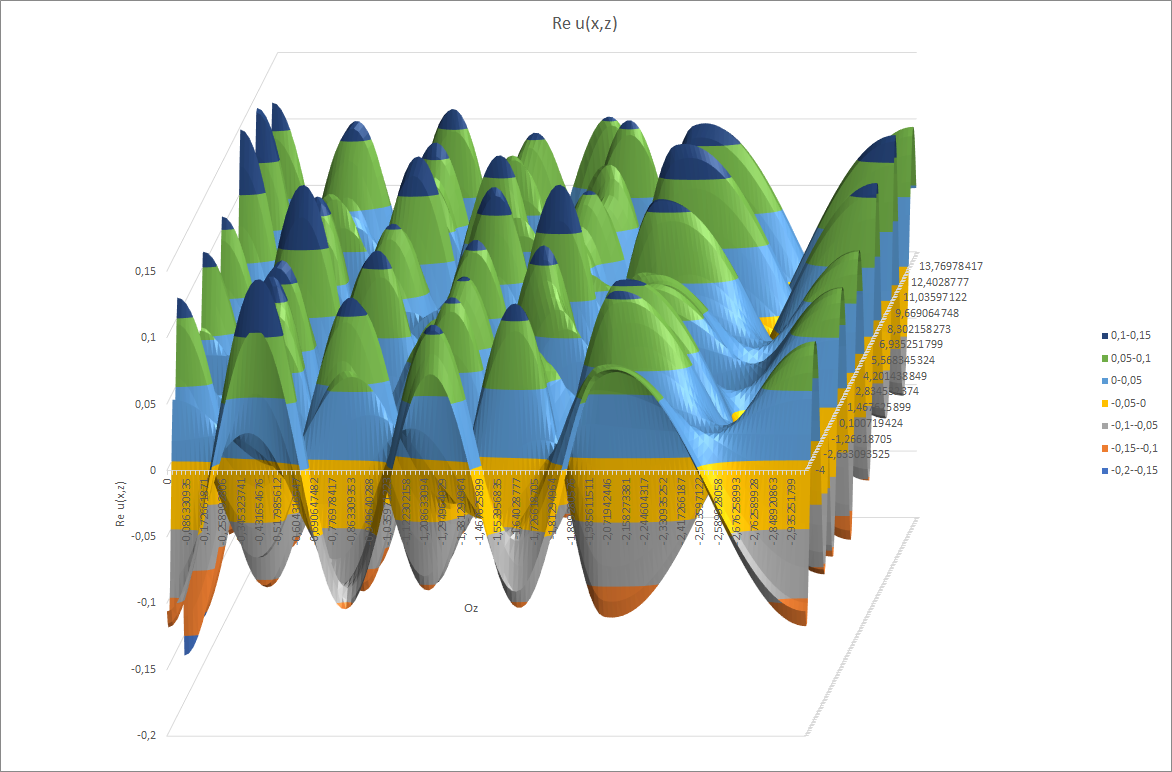
\includegraphics[width=0.95\linewidth]{109.png}
}
\caption{Действительная часть $u(x,z), x \in [-4;15], z\in [-3;0], c_1=h_2=\mu_1=1, \mu_2=c_2=h_2=2, \omega=8$}
\label{figCurves}
\end{figure}        


\end{document}